
\section{Three Dimensional Plot Types}
\label{sec:3d}

{
\tikzset{external/figure name/.add={}{threedim_}}

\PGFPlots{} provides three dimensional visualizations like scatter, line, mesh
or surface plots. This section explains the methods to provide input
coordinates and how to use the different plot types.


\subsection{Before You Start With 3D}
\label{pgfplots:3d:preliminary}

Before we delve into the capabilities of \PGFPlots{} for three dimensional
visualization, let me start with some preliminary remarks. The reason to use
\PGFPlots{} for three dimensional plots are similar to those of normal, two
dimensional plots: the possibility to get consistent fonts and document
consistent styles combined with high-quality output.

While this works very nice for (not too complex) two dimensional plots, it
requires considerably more effort than non-graphical documents. This is even
more so for three dimensional plots. In other words: \PGFPlots{}' three
dimensional routines are slow. There are reasons for this and some of them may
vanish in future versions. But one of these reasons is that \TeX{} has never
been designed for complex visualisation techniques. Consider using |lualatex|
(and at least |compat=1.12|) in order to reduce compilation times and to avoid
memory limitations. Also consider the image externalization routines mentioned
in Section~\ref{sec:pgfplots:export}, in particular the |external| library to
reduce typesetting time. Besides the speed limitations, three dimensional plots
reach memory limits easily. Therefore, the plot complexity of three dimensional
plots is limited to relatively coarse resolutions.
Section~\ref{sec:pgfplots:export} also discusses methods to extend the initial
\TeX{} memory limits.

Another issue which arises in three dimensional visualization is depth: it is
necessary to decide which items are to be drawn in front of others. \PGFPlots{}
supports $z$ buffering techniques up to a certain extend: it works pretty well
for single scatter plots (|z buffer=sort|), mesh or surface plots
(|z buffer=auto|) or parametric mesh and surface plots (|z buffer=sort|).
However, it cannot combine different |\addplot| commands, those will be drawn in
the order of appearance. You may encounter the limitations sometimes. Maybe it
will be improved in future versions.

If you decide that you need high complexity, speed and 100\% reliable z buffers
(depth information), you should consider using other visualization tools and
return to \PGFPlots{} in several years. If you can wait for a complex picture
and you do not even see the limitations arising from z buffering limitations,
you should use \PGFPlots{}. Again, consider using the automatic picture
externalization with the |external| library discussed in
Section~\ref{sec:pgfplots:export}.


\subsection{The \texttt{\textbackslash addplot3} Command: Three Dimensional Coordinate Input}
\label{pgfplots:sec:threedim}

\begin{addplot3generic}
    The \verbpdfref{\addplot3} command is the main interface for any three
    dimensional plot. It works in the same way as its two dimensional variant
    |\addplot| which has been described in all detail in
    Section~\ref{cmd:pgfplots:addplot} on page~\pageref{cmd:pgfplots:addplot}.

    The \verbpdfref{\addplot3} command accepts the same input methods as the
    |\addplot| variant, including expression plotting, coordinates, files and
    tables. However, a third coordinate is necessary for each of these methods
    which is usually straightforward and is explained in all detail in the
    following.

    Furthermore, \verbpdfref{\addplot3} has a way to decide whether a
    \emph{line} visualization or a \emph{mesh} visualization has to be
    done\index{3d: line or mesh}. The first one is a map from one dimension
    into $\R^3$ and the latter one a map from two dimensions to $\R^3$. Here,
    the keys |mesh/rows| and |mesh/cols| are used to define mesh sizes (matrix
    sizes). Usually, you don't have to care about that because the coordinate
    input routines already allow either one- or two-dimensional structure.

    The precise rules how \PGFPlots{} distinguishes between line visualization
    and mesh visualization is as follows:
    %
    \begin{enumerate}
        \item If the key |mesh input=patches| has been used, \PGFPlots{}
            relies on the current |patch type| (which has an inherent
            dimension).
        \item For all other values of |mesh input| (like |mesh input=lattice|
            and |mesh input=image|), \PGFPlots{} proceeds as follows:
            %
            \begin{itemize}
                \item It auto-completes the values for |mesh/rows| and
                    |mesh/cols| (or uses their prescribed values).
                \item If these keys describe a matrix of size $1\times N$
                    or $N \times 1$, \PGFPlots{} assumes that it is a line.
            \end{itemize}

            The ``auto-completion'' depends on how you provide your data.
            %
            \begin{itemize}
                \item If you use \verbpdfref{\addplot3 expression},
                    |mesh/rows| and |mesh/cols| are computed from the
                    values |samples| and |samples y|. By default,
                    \verbpdfref{\addplot3 expression} always samples a
                    mesh. If you want it to sample a line, set
                    |samples y=1| (or, equivalently, |y domain=0:0|).
                \item If you use \verbpdfref{\addplot3 table},
                    \verbpdfref{\addplot3 coordinates}, or
                    \verbpdfref{\addplot3 file}, you have basically two
                    options: either you provide at least one of |mesh/rows|
                    or |mesh/cols| explicitly, or you format the input
                    table by means of end-of-scanline markers as outlined
                    in |empty line=auto| or |empty line=scanline|. In this
                    case, \PGFPlots{} counts scanline lengths and uses
                    |mesh/ordering| to conclude how to determine the matrix
                    values.

                    Thus, if you have empty lines in your input table,
                    \PGFPlots{} will automatically identify the matrix size.

                    If you do \emph{not} have empty lines, \PGFPlots{} expects
                    at least one of |mesh/rows| or |mesh/cols|.
            \end{itemize}
    \end{enumerate}
\end{addplot3generic}

\begin{addplot3operation}[]{coordinates}{\marg{coordinate list}}
    The \verbpdfref{\addplot3 coordinates} method works like its
    two-dimensional variant, \verbpdfref{\addplot coordinates} which is
    described in all detail on page~\pageref{pgfplots:addplot:coordinates}:

    A long list of coordinates |(|\meta{x}|,|\meta{y}|,|\meta{z}|)| is
    expected, separated by white spaces. The input list can be either an
    unordered series of coordinates, for example for scatter or line plots. It
    can also have matrix structure, in which case an |empty line| (which is
    equivalent to ``|\par|'') marks the end of one matrix row. Matrix structure
    can also be provided if one of |mesh/rows| or |mesh/cols| is provided
    explicitly.

\begin{codeexample}[]
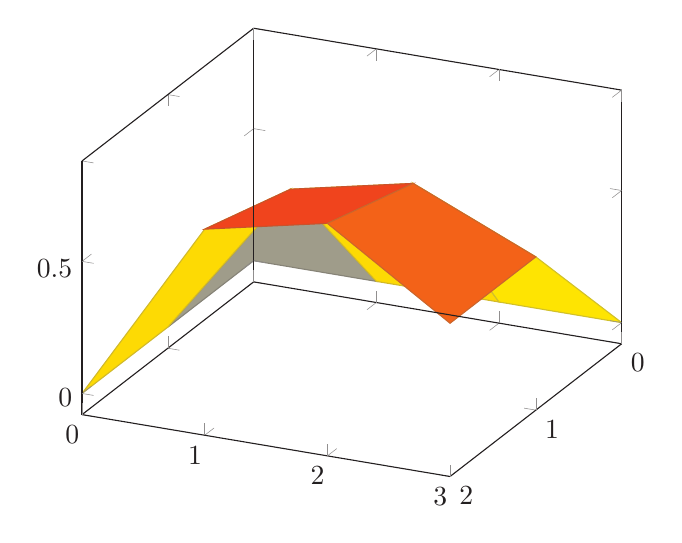
\begin{tikzpicture}
\begin{axis}
    % this yields a 3x4 matrix:
    \addplot3 [surf] coordinates {
        (0,0,0) (1,0,0)   (2,0,0)   (3,0,0)

        (0,1,0) (1,1,0.6) (2,1,0.7) (3,1,0.5)

        (0,2,0) (1,2,0.7) (2,2,0.8) (3,2,0.5)
    };
\end{axis}
\end{tikzpicture}
\end{codeexample}
    %
    \noindent Here, \verbpdfref{\addplot3} reads a matrix with three rows and
    four columns. The |empty line|s separate one row from the following.

    As for the two-dimensional |\addplot coordinates|, it is possible to provide
    (constant) mathematical expressions inside of single coordinates. The
    syntax |(|\meta{x}|,|\meta{y}|,|\meta{z}|) |\oarg{meta} can be used just as
    for two dimensional |\addplot coordinates| to provide explicit color data;
    error bars are also supported.
\end{addplot3operation}

\begin{addplot3operation}[]{table}{\oarg{column selection}\marg{file}}
    The \verbpdfref{\addplot3 table} input works in the same way as its two
    dimensional counterpart \verbpdfref{\addplot table}. It only expects a
    column for the $z$-coordinates.

    As for \verbpdfref{\addplot3 coordinates}, an |empty line| in the file
    marks the end of one matrix row.

    For matrix data in files, it is important to specify the ordering in which
    the matrix entries have been written. The default configuration is
    |mesh/ordering=x varies|, so you need to change it to
    |mesh/ordering=y varies| in case you have column by column ordering.

\begin{codeexample}[]
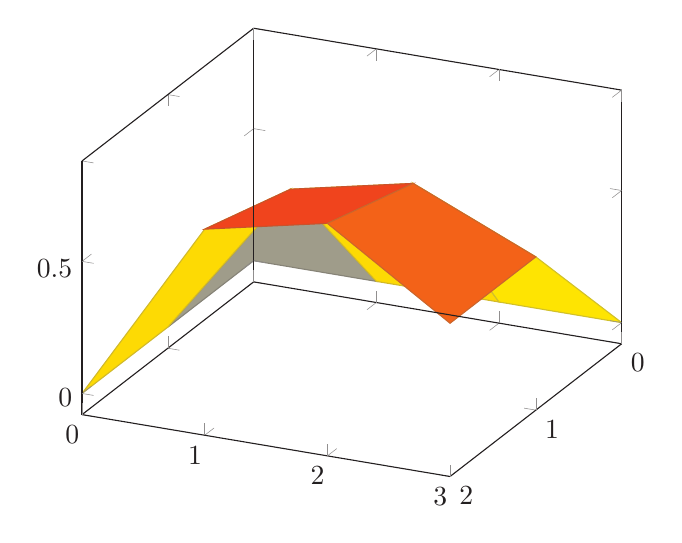
\begin{tikzpicture}
\begin{axis}
    % this yields a 3x4 matrix:
    \addplot3 [surf] table {
         0 0 0
         1 0 0
         2 0 0
         3 0 0

         0 1 0
         1 1 0.6
         2 1 0.7
         3 1 0.5

         0 2 0
         1 2 0.7
         2 2 0.8
         3 2 0.5
    };
\end{axis}
\end{tikzpicture}
\end{codeexample}
\end{addplot3operation}

\begin{addplot3operation}[]{file}{\marg{name}}
    \paragraph{Deprecation note:}

    If you have data files, you should generally use |\addplot table|. The
    input type |\addplot file| is almost the same, but considerably less
    powerful. It is only kept for backwards compatibility.

    The \verbpdfref{\addplot3 file} input method is the same as
    \verbpdfref{\addplot file} -- it only expects one more coordinate. Thus,
    the input file contains $x_i$ in the first column, $y_i$ in the second
    column and $z_i$ in the third.

    A further column is read after $z_i$ if |point meta=explicit| has been
    requested, see the documentation of \verbpdfref{\addplot file} on
    page~\pageref{pgfplots:addplot:file} for details.

    As for \verbpdfref{\addplot3 coordinates}, an |empty line| in the file
    marks the end of one matrix row.
    %
\begin{codeexample}[]
\begin{tikzpicture}
\begin{axis}
    % We have `plotdata/first3d.dat' with
    %---------
    % 0 0 0.8
    % 1 0 0.56
    % 2 0 0.5
    % 3 0 0.75
    %
    % 0 1 0.6
    % 1 1 0.3
    % 2 1 0.21
    % 3 1 0.3
    %
    % 0 2 0.68
    % 1 2 0.22
    % 2 2 0.25
    % 3 2 0.4
    %
    % 0 3 0.7
    % 1 3 0.5
    % 2 3 0.58
    % 3 3 0.9
    % -> yields a 4x4 matrix:
    \addplot3 [surf] file {plotdata/first3d.dat};
\end{axis}
\end{tikzpicture}
\end{codeexample}

    For matrix data in files, it is important to specify the ordering in which
    the matrix entries have been written. The default configuration is
    |mesh/ordering=x varies|, so you need to change it to
    |mesh/ordering=y varies| in case you have column by column ordering.
\end{addplot3operation}

\begin{pgfplotskeylist}{mesh/rows=\marg{integer},mesh/cols=\marg{integer}}
    For visualization of mesh or surface plots which need some sort of matrix
    input, the dimensions of the input matrix need to be known in order to
    visualize the plots correctly. The matrix structure may be known from
    end-of-row marks (|empty line|s as general end-of-scanline markers in the
    input stream) as has been described above.

    If the matrix structure is not yet known, it is necessary to provide at
    least one of |mesh/rows| or |mesh/cols| where |mesh/rows| indicates the
    number of samples for $y$-coordinates whereas |mesh/cols| is the number of
    samples used for $x$-coordinates (see also |mesh/ordering|).

    Thus, the following example is also a valid method to define an input
    matrix.
    %
\begin{codeexample}[]
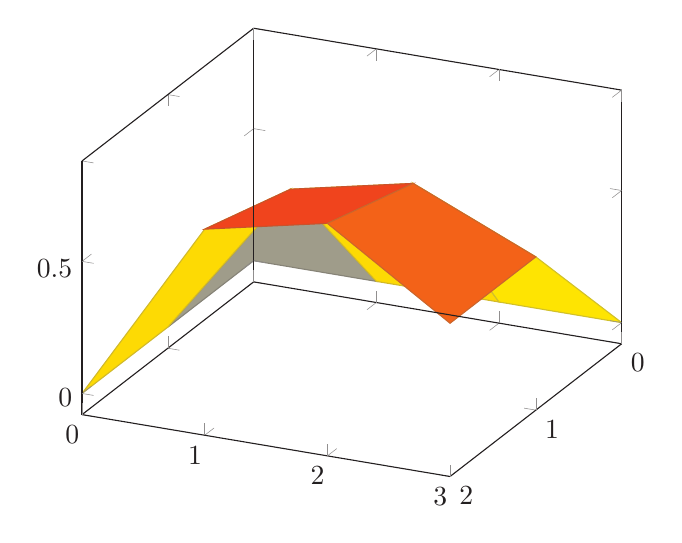
\begin{tikzpicture}
\begin{axis}
    % this yields also a 3x4 matrix:
    \addplot3 [surf,mesh/rows=3] coordinates {
        (0,0,0) (1,0,0)   (2,0,0)   (3,0,0)
        (0,1,0) (1,1,0.6) (2,1,0.7) (3,1,0.5)
        (0,2,0) (1,2,0.7) (2,2,0.8) (3,2,0.5)
    };
\end{axis}
\end{tikzpicture}
\end{codeexample}

    It is enough to supply one of |mesh/rows| or |mesh/cols| -- the missing
    value will be determined automatically.

    If you provide one of |mesh/rows| or |mesh/cols|, any end-of-row marker
    seen inside of input files or coordinate streams will be ignored.
\end{pgfplotskeylist}

\begin{pgfplotskeylist}{mesh/scanline verbose=\mchoice{true,false} (initially false)}
    Provides debug messages in the \LaTeX{} output about end-of-scanline
    markers.

    The message will tell whether end-of-scanlines have been found and if they
    are the same.
\end{pgfplotskeylist}

\begin{pgfplotskey}{mesh/ordering=\mchoice{x varies,y varies,rowwise,colwise} (initially x varies)}
    Allows to configure the sequence in which matrices (meshes) are read from
    \verbpdfref{\addplot3 coordinates}, \verbpdfref{\addplot3 file} or
    \verbpdfref{\addplot3 table}.

    Here, \declaretext{x varies} means a sequence of points where
    $n$=|mesh/cols| successive points have the $y$-coordinate fixed. This is
    intuitive when you write down a function because $x$ is horizontal and $y$
    vertical. Note that in matrix terminology, $x$ refers to \emph{column
    indices} whereas $y$ refers to \emph{row indices}. Thus, |x varies| is
    equivalent to \declaretext{rowwise} ordering in this sense. This is the
    initial configuration.

\begin{codeexample}[]
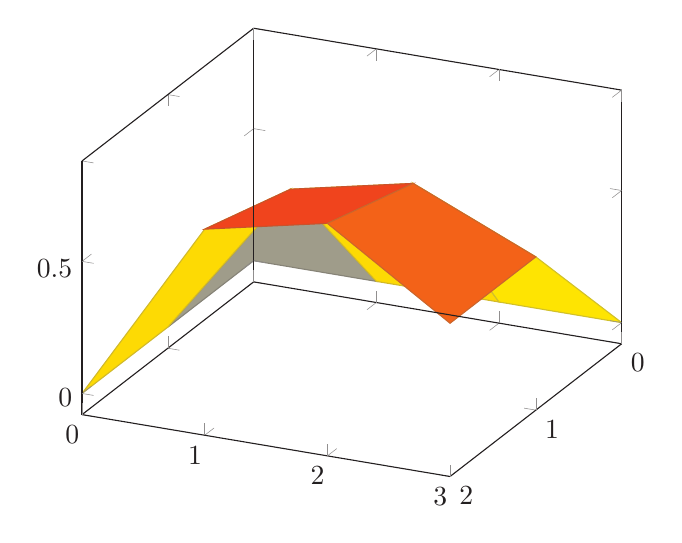
\begin{tikzpicture}
\begin{axis}[mesh/ordering=x varies]
    % this yields a 3x4 matrix in `x varies'
    % ordering:
    \addplot3 [surf] coordinates {
        (0,0,0) (1,0,0)   (2,0,0)   (3,0,0)

        (0,1,0) (1,1,0.6) (2,1,0.7) (3,1,0.5)

        (0,2,0) (1,2,0.7) (2,2,0.8) (3,2,0.5)
    };
\end{axis}
\end{tikzpicture}
\end{codeexample}
    %
    \noindent Note that |mesh/ordering| is mandatory, even though the size of
    the matrix can be provided in different ways. The example above uses
    |empty line|s to mark scanlines. One could also say |mesh/rows=3| and omit
    the |empty line|s.

    Consequently, |mesh/ordering=|\declaretext{y varies} provides points such
    that successive $m$=|mesh/rows| points form a column, i.e.\@ the
    $x$-coordinate is fixed and the $y$-coordinate changes. In this sense,
    |y varies| is equivalent to \declaretext{colwise} ordering, it is actually
    a matrix transposition.
    %
\begin{codeexample}[]
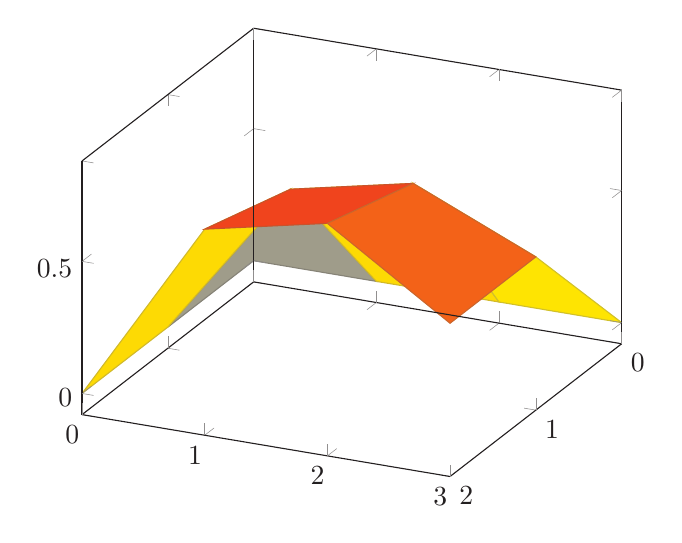
\begin{tikzpicture}
\begin{axis}[mesh/ordering=y varies]
    % this yields a 3x4 matrix in column-wise ordering:
    \addplot3 [surf] coordinates {
        (0,0,0) (0,1,0)   (0,2,0)

        (1,0,0) (1,1,0.6) (1,2,0.7)

        (2,0,0) (2,1,0.7) (2,2,0.8)

        (3,0,0) (3,1,0.5) (3,2,0.5)
    };
\end{axis}
\end{tikzpicture}
\end{codeexample}
    %
    Again, note the subtle difference to the common matrix indexing where a
    column has the second index fixed. \PGFPlots{} refers to the way one would
    write down a function on a sheet of paper (this is consistent with how
    Matlab$^\text{\textregistered}$ displays discrete functions with matrices).
\end{pgfplotskey}

\begin{addplot3operation}[]{\marg{math expression}}{}
\label{cmd:addplot3:expr}
        \pgfmanualpdflabel{\textbackslash addplot3 expression}{}%
    Expression plotting also works in the same way as for two dimensional
    plots. Now, however, a two dimensional mesh is sampled instead of a single
    line, which may depend on |x| and |y|.

    The method \verbpdfref{\addplot3} \marg{math expr} visualizes the function
    $f(x,y) = $\meta{math expr} where $ f \colon [x_1,x_2] \times [y_1,y_2] \to
    \R$. The interval $[x_1,x_2]$ is determined using the |domain| key, for
    example using |domain=0:1|. The interval $[y_1,y_2]$ is determined using
    the |y domain| key. If |y domain| is empty, $[y_1,y_2] = [x_1,x_2]$ will be
    assumed. If |y domain=0:0| (or any other interval of length zero), it is
    assumed that the plot does not depend on |y| (thus, it is a line plot).

    The number of samples in $x$ direction is set using the |samples| key. The
    number of samples in $y$ direction is set using the |samples y| key. If
    |samples y| is not set, the same value as for $x$ is used. If
    |samples y|$\,\le 1$, it is assumed that the plot does not depend on |y|
    (meaning it is a line plot).

\pgfplotsexpensiveexample
\begin{codeexample}[]
% requires \usepgfplotslibrary{colorbrewer}
\begin{tikzpicture}
\begin{axis}[
    colormap/PuBu,
]
    \addplot3 [surf] {y};
\end{axis}
\end{tikzpicture}
\end{codeexample}

\pgfplotsexpensiveexample
\begin{codeexample}[]
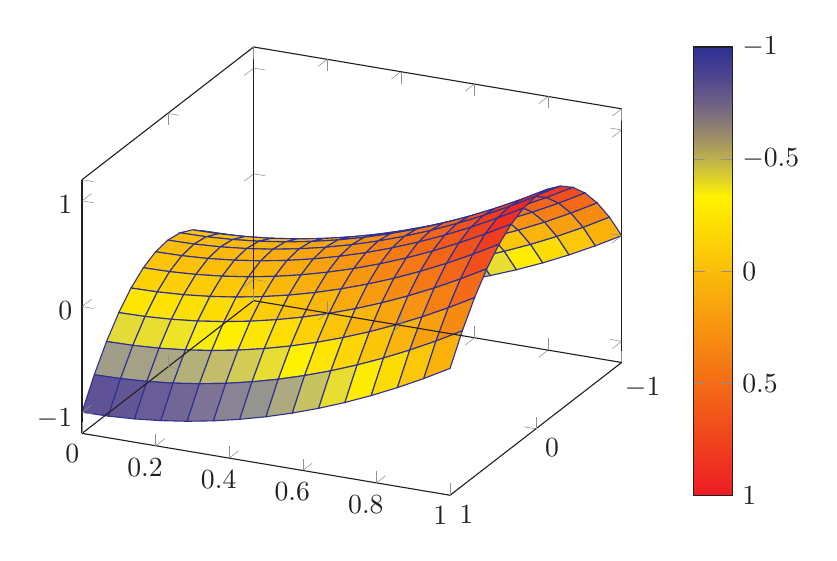
\begin{tikzpicture}
\begin{axis}[colorbar]
    \addplot3 [
        surf,
        faceted color=blue,
        samples=15,
        domain=0:1,y domain=-1:1
    ] {x^2 - y^2};
\end{axis}
\end{tikzpicture}
\end{codeexample}

    Expression plotting sets |mesh/rows| and |mesh/cols| automatically; these
    settings don't have any effect for expression plotting.
\end{addplot3operation}

\begin{addplot3operation}[]{expression}{\marg{math expression}}
    The syntax

    \verbpdfref{\addplot3} \marg{math expression}|;|

    as short-hand equivalent for

    \verbpdfref{\addplot3 expression} \marg{math expression}|;|
\end{addplot3operation}

\begin{addplot3operation}[]{(\meta{$x$ expression},\meta{$y$ expression},\meta{$z$ expression})}{}
    A variant of \verbpdfref{\addplot3 expression} which allows to provide
    different coordinate expressions for the $x$-, $y$- and $z$-coordinates.
    This can be used to generate parameterized plots.

    Please note that |\addplot3 (x,y,x^2)| is equivalent to
    |\addplot3 expression {x^2}|.

    Note further that since the complete point expression is surrounded by
    round braces, round braces inside of \meta{$x$ expression}, \meta{$y$
    expression} or \meta{$z$ expression} need to be treated specially. Surround
    the expressions (which contain round braces) with curly braces:

    |\addplot3 (|\marg{$x$ expr}|, |\marg{$y$ expr}|, |\marg{$z$ expr}|);|
\end{addplot3operation}


\subsection{Line Plots}
\label{sec:pgfplots:lineplots}

Three dimensional line plots are generated if the input source has no matrix
structure. Line plots take the input coordinates and connect them in the order
of appearance.

\begin{codeexample}[]
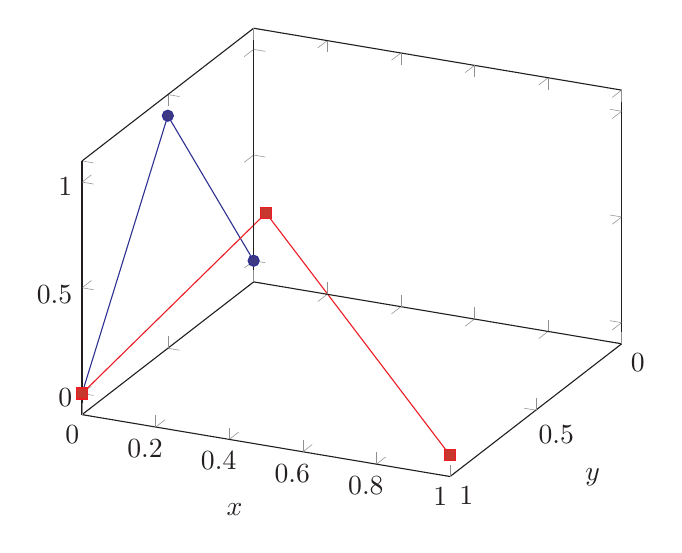
\begin{tikzpicture}
\begin{axis}[
    xlabel=$x$,
    ylabel=$y$,
]
    \addplot3 coordinates {(0,0,0) (0,0.5,1) (0,1,0)};
    \addplot3 coordinates {(0,1,0) (0.5,1,1) (1,1,0)};
\end{axis}
\end{tikzpicture}
\end{codeexample}
%
If there is no value for neither |mesh/rows| nor |mesh/cols| or if one of them
is |1|, \PGFPlots{} will draw a line plot. This is also the case if there is no
end-of-scanline marker (|empty line|) in the input stream.

For \verbpdfref{\addplot3 expression}, this requires to set |samples y=1| to
disable the generation of a mesh.
%
\begin{codeexample}[]
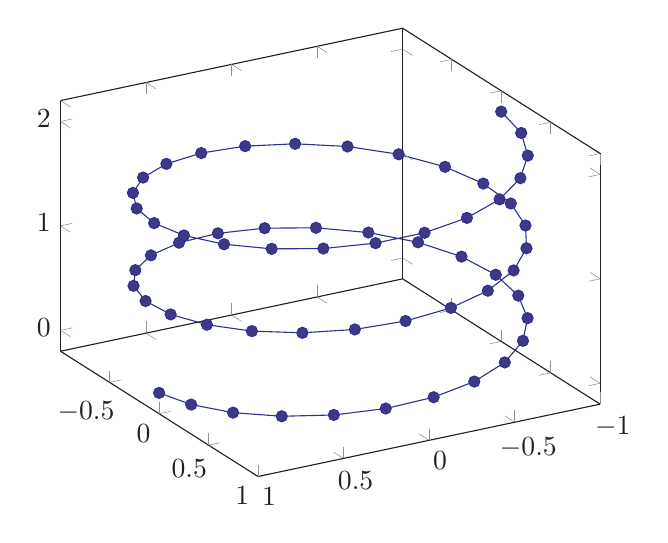
\begin{tikzpicture}
\begin{axis}[view={60}{30}]
    \addplot3+ [
        domain=0:5*pi,
        samples=60,
        samples y=0,
    ] (
        {sin(deg(x))},
        {cos(deg(x))},
        {2*x/(5*pi)}
    );
\end{axis}
\end{tikzpicture}
\end{codeexample}
%
\noindent The example above is a parametric plot by expression, i.e.\@ it has
three distinct expressions for $x$, $y$, and $z$.

Line plots in three dimensions are also possible for data plots (tables). The
most simple case is if you simply provide a series of three-dimensional
coordinates which will be connected in the order of appearance:
%
\begin{codeexample}[]
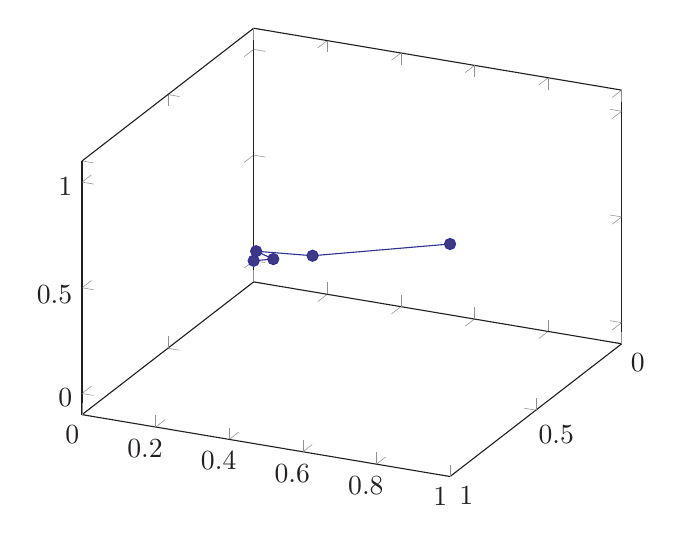
\begin{tikzpicture}
\begin{axis}
    \addplot3 table {
        x   y   z
        0   0   0
        0.1 0.1 0.1
        0.1 0.2 0.2
        0.3 0.3 0.3
        1   1   1
    };
\end{axis}
\end{tikzpicture}
\end{codeexample}
%
\noindent Note that this plot implicitly has |mesh/rows=1| because it has no
end-of-scanline markers (|empty line|s). If in doubt, you can set |mesh/rows=1|
explicitly to tell \PGFPlots{} that you have one-dimensional data (and not a
matrix).

Line plots from data files are also possible if the data files only contains
two coordinates -- and the third should be provided somehow. In this case, the
|table/x expr| feature comes into play: it allows to combine data plots and
math expressions:
%
\begin{codeexample}[]
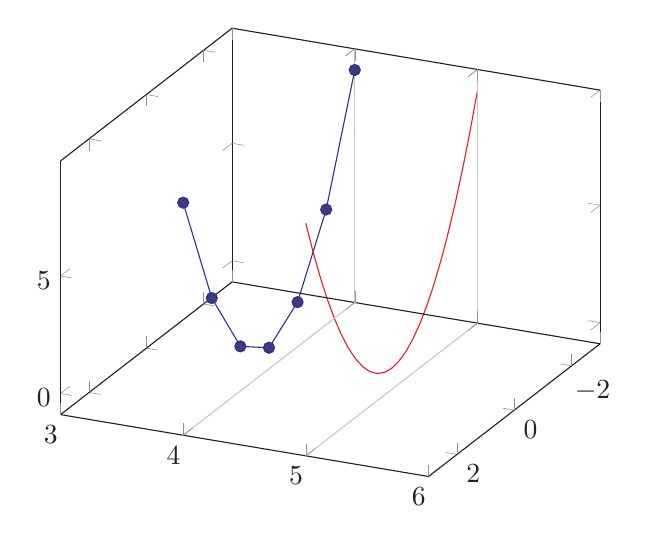
\begin{tikzpicture}
\begin{axis}[
    xmin=3,xmax=6,
    extra x ticks={4,5},
    extra x tick style={xticklabel=\empty,grid=major}
]
    \addplot3 table [x expr=4,y=a,z=b] {
        a  b
        -3 9
        -2 4
        -1 1
        0  0
        1  1
        2  4
        3  9
    };
    \addplot3 [red,domain=-3:3,samples y=1] (5,x,x^2);
\end{axis}
\end{tikzpicture}
\end{codeexample}
%
\noindent Here, we have two plots in one axis: one data plot from a data table
with just two coordinates and one parametric plot. Both denote the same two
functions. For the data plot, |x expr=4| assigns the $x$-coordinate, and
|y=a,z=b| define how the input columns map to coordinates. Again, the plot
implicitly uses |mesh/rows=1| since there is no end-of-scanline marker. The
second plot does the same with the short-handed notation |(5,x,x^2)|. It only
samples one-dimensional data due to |samples y=1|. Finally, |extra x ticks|
configures two additional ticks for the $x$-axis; this is used to display grid
lines for these specific ticks. The |xticklabel=\empty| argument avoids
overprinted $x$~tick labels at positions $x\in\{4,5\}$.

Three dimensional line plots will usually employ lines to connect points
(i.e.\@ the initial |sharp plot| handler of \Tikz). The |smooth| method of
\Tikz{} might also prove be an option. Note that no piecewise constant plot,
comb or bar plot handler is supported for three dimensional axes.


\subsubsection{Filled Lined Plots in 3D}
\label{sec:pgfplots:filled:line}

Closing a line plot is also possible for three-dimensional axes. This works in
the same way as outlined in Section~\ref{sec:pgfplots:closingplots} for
two-dimensional axes: by using |\closedcycle|.

\begin{codeexample}[]
\begin{tikzpicture}
\pgfplotstableread{
plot1     plot2     plot3     plot4
0.0045    0.0029    0.0089    0.0001
0.0024    0.0023    0.0050    0.0016
0.0007    0.0012    0.0010    0.0001
0.0000    0.0004   -0.0000   -0.0015
0.0001    0.0001    0.0007   -0.0021
0.0003    0.0000    0.0015   -0.0020
0.0003    0.0001    0.0017   -0.0018
0.0003    0.0001    0.0016   -0.0015
0.0003    0.0001    0.0016   -0.0013
0.0003    0.0002    0.0015   -0.0012
}\tabledata
\begin{axis}[
    zmin=-0.001,
    area plot/.style={
        fill opacity=0.75,
        draw=orange!80!black,thick,
        fill=orange,
        mark=none,
    },
    ytick={1,...,4},
    yticklabel=plot\pgfmathprintnumber{\tick},
]
    \pgfplotsinvokeforeach{4,3,...,1}{
        \addplot3 [area plot] table [
            x expr=\coordindex, y expr=#1, z=plot#1,
        ] {\tabledata} \closedcycle;
    }
\end{axis}
\end{tikzpicture}
\end{codeexample}

The difference here is that \PGFPlots{} will connect the first and last
coordinates on the $z=0$ plane, or, if $z=0$ is outside of the axis limits, on
the plane $z_{\min}$.


\subsection{Scatter Plots}

Three dimensional scatter plots have the same interface as for two dimensional
scatter plots, so all examples of Section~\ref{sec:pgfplots:scatter:2d} can be
used for the three dimensional case as well. The key features are to use
|only marks| and/or |scatter| as plot styles.

We provide some more examples which are specific for the three dimensional case.

Our first example uses |only marks| to place the current plot |mark| at each
input position:
%
\pgfplotsexpensiveexample
\begin{codeexample}[]
\begin{tikzpicture}
\begin{axis}[
    xlabel=$x$,
    ylabel=$y$,
    zlabel={$f(x,y) = x\cdot y$},
    title=A Scatter Plot Example,
]
    % `pgfplotsexample4_grid.dat' contains a
    % large sequence of input points of the form
    % x_0   x_1     f(x)
    % 0     0       0
    % 0     0.03125 0
    % 0     0.0625  0
    % 0     0.09375 0
    % 0     0.125   0
    % 0     0.15625 0
    \addplot3+ [only marks]
        table {plotdata/pgfplotsexample4_grid.dat};
    \end{axis}
\end{tikzpicture}
\end{codeexample}

If we add the key |scatter|, the plot mark will also use the colors of the
current |colormap|:
%
\pgfplotsexpensiveexample
\begin{codeexample}[]
\begin{tikzpicture}
\begin{axis}[
    xlabel=$x$,
    ylabel=$y$,
    zlabel={$f(x,y) = x\cdot y$},
    title=A Scatter Plot Example,
]
    \addplot3+ [
        only marks,
        scatter,
    ] table {plotdata/pgfplotsexample4_grid.dat};
\end{axis}
\end{tikzpicture}
\end{codeexample}

A more sophisticated example is to draw the approximated function as a |surf|
plot (which requires matrix data) and the underlying grid (which is |scatter|ed
data) somewhere into the same axis. We choose to place the $(x,y)$ grid points
at $z=1.4$. Furthermore, we want the grid points to be colored according to the
value of column |f(x)| in the input table:

\pgfplotsexpensiveexample
\begin{codeexample}[]
\begin{tikzpicture}
    \begin{axis}[
        3d box,
        zmax=1.4,
        colormap/viridis,
        colorbar,
        xlabel=$x$,
        ylabel=$y$,
        zlabel={$f(x,y) = x\cdot y$},
        title={Using Coordinate Filters to fix $z=1.4$},
    ]
        % `pgfplotsexample4.dat' contains similar data as in
        % `pgfplotsexample4_grid.dat', but it uses a uniform
        % matrix structure (same number of points in every scanline).
        % See examples above for extracts.
        \addplot3 [surf,mesh/ordering=y varies]
            table {plotdata/pgfplotsexample4.dat};
        \addplot3 [scatter,scatter src=\thisrow{f(x)},only marks, z filter/.code={\def\pgfmathresult{1.4}}]
            table {plotdata/pgfplotsexample4_grid.dat};
    \end{axis}
\end{tikzpicture}
\end{codeexample}
%
\noindent We used |z filter| to fix the $z$-coordinate to $1.4$. We could also
have used the |table/z expr=1.4| feature
%
\begin{codeexample}[code only]
    \addplot3 [scatter,scatter src=\thisrow{f(x)},only marks]
        table [z expr=1.4] {plotdata/pgfplotsexample4_grid.dat};
\end{codeexample}
%
\noindent to get exactly the same effect. Choose whatever you like best. The
|z filter| works for every coordinate input routine, the |z expr| feature is
only available for |\addplot table|.

The following example uses |mark=cube*| and |z buffer=sort| to place boxes at
each input coordinate. The color for each box is determined by
|point meta={x+y+3}|. The remaining keys are just for pretty printing.
%
\pgfplotsexpensiveexample
\begin{codeexample}[]
\begin{tikzpicture}
    \begin{axis}[
        view={120}{40},
        width=220pt,
        height=220pt,
        grid=major,
        z buffer=sort,
        xmin=-1,xmax=9,
        ymin=-1,ymax=9,
        zmin=-1,zmax=9,
        enlargelimits=upper,
        xtick={-1,1,...,19},
        ytick={-1,1,...,19},
        ztick={-1,1,...,19},
        xlabel={$l_1$},
        ylabel={$l_2$},
        zlabel={$l_3$},
        point meta={x+y+z+3},
        colormap={summap}{
            color=(black)  color=(blue)
            color=(black)  color=(white)
            color=(orange) color=(violet)
            color=(red)
        },
        scatter/use mapped color={
            draw=mapped color,fill=mapped color!70},
        ]
        % `pgfplots_scatter4.dat' contains a large sequence of
        % the form
        % l_0   l_1     l_2
        % 1     6       -1
        % -1    -1      -1
        % 0     -1      -1
        % -1    0       -1
        % -1    -1      0
        % 1     -1      -1
        % 0     0       -1
        % 0     -1      0
        \addplot3 [only marks,scatter,mark=cube*,mark size=7]
            table {plotdata/pgfplots_scatterdata4.dat};
    \end{axis}
\end{tikzpicture}
\end{codeexample}


\subsection{Mesh Plots}
\label{sec:2d:mesh}

\begin{plottype}[/pgfplots]{mesh}
    A mesh plot uses different colors for each mesh segment. The color is
    determined using a ``color coordinate'' which is also called ``meta data''
    throughout this document. It is the same data which is used for surface and
    scatter plots as well, see Section~\ref{pgfplots:pointmeta}. In the initial
    configuration, the ``color coordinate'' is the $z$-axis (or the $y$-axis
    for two dimensional plots). This color coordinate is mapped linearly into
    the current color map to determine the color for each mesh segment. Thus,
    if the smallest occurring color data is, say, $-1$ and the largest is $42$,
    points with color data $-1$ will get the color at the lower end of the
    color map and points with color data $42$ the color of the upper end of the
    color map.

\pgfplotsexpensiveexample
\begin{codeexample}[]
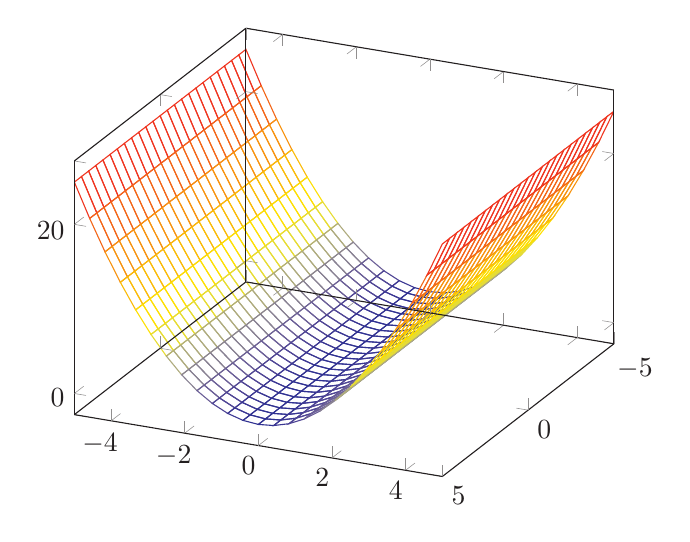
\begin{tikzpicture}
\begin{axis}
    \addplot3 [mesh] {x^2};
\end{axis}
\end{tikzpicture}
\end{codeexample}

    A mesh plot can be combined with markers or with the |scatter| key which
    also draws markers in different colors.

\pgfplotsexpensiveexample
\begin{codeexample}[]
% requires \usepgfplotslibrary{colorbrewer}
\begin{tikzpicture}
\begin{axis}[
    colormap/PuOr,
]
    \addplot3+ [
        mesh,
        scatter,
        samples=10,
        domain=0:1,
    ] {x*(1-x)*y*(1-y)};
\end{axis}
\end{tikzpicture}
\end{codeexample}

\pgfplotsexpensiveexample
\begin{codeexample}[]
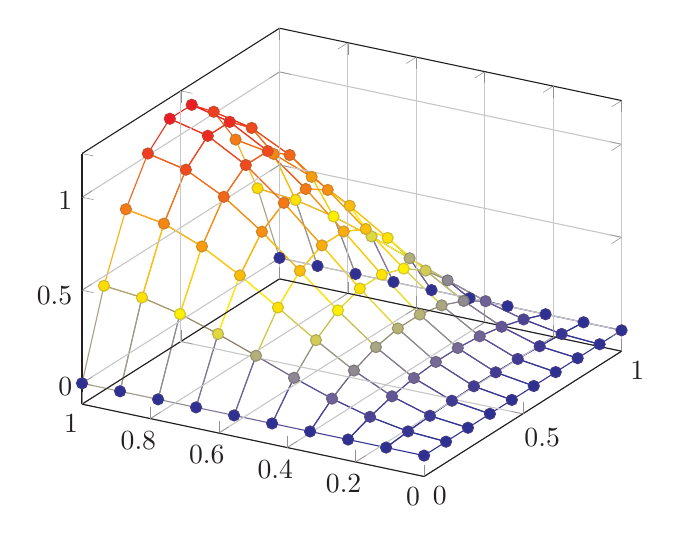
\begin{tikzpicture}
\begin{axis}[
    grid=major,
    view={210}{30},
]
    \addplot3+ [
        mesh,
        scatter,
        samples=10,
        domain=0:1,
    ] {5*x*sin(2*deg(x)) * y*(1-y)};
\end{axis}
\end{tikzpicture}
\end{codeexample}

    Occasionally, one may want to hide the background mesh segments. This can
    be achieved using the |surf| plot handler (see below) and a specific fill
    color:
    %
\pgfplotsexpensiveexample
\begin{codeexample}[]
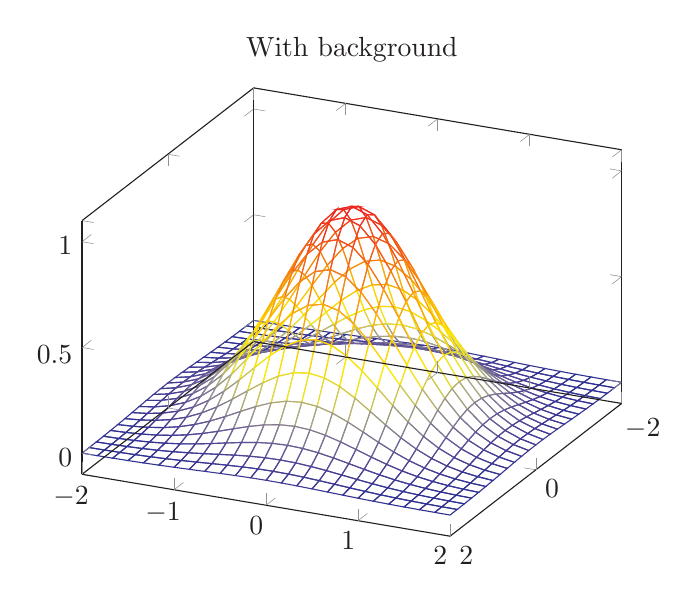
\begin{tikzpicture}
    \begin{axis}[title=With background]
        \addplot3 [mesh,domain=-2:2] {exp(-x^2-y^2)};
    \end{axis}
\end{tikzpicture}
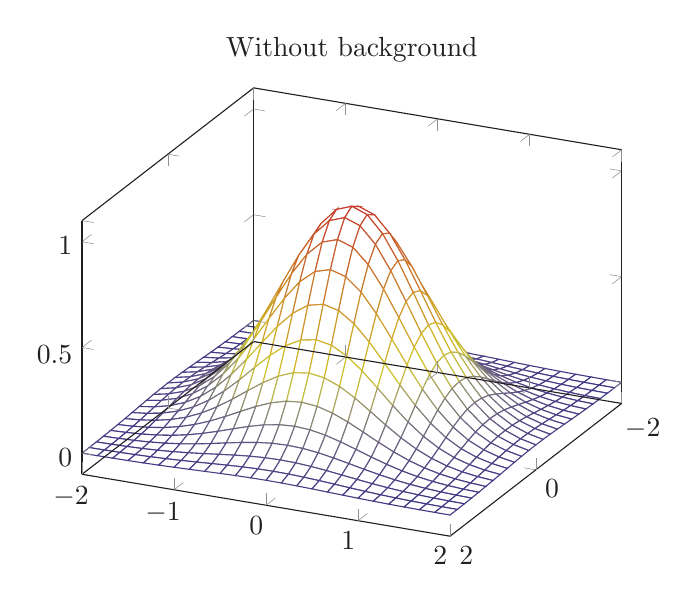
\begin{tikzpicture}
    \begin{axis}[title=Without background]
        \addplot3 [surf,fill=white,domain=-2:2] {exp(-x^2-y^2)};
    \end{axis}
\end{tikzpicture}
\end{codeexample}
    %
    The fill color needs to be provided explicitly.


    \paragraph{Details:}

    \begin{itemize}
        \item A mesh plot uses the same implementation as |shader=flat| to
            get one color for each single segment. Thus, if
            |shader=flat mean|, the color for a segment is determined using
            the \emph{mean} of the color data of adjacent vertices. If
            |shader=flat corner|, the color of a segment is the color of
            \emph{the first} adjacent vertex.\footnote{Starting with
            \PGFPlots{} 1.13 and the associated compatibility level, this
            holds even in the presence of $z$ buffering.}
        \item As soon as |mesh| is activated, |color=mapped color| is
            installed. This is \emph{necessary} unless one needs a different
            color -- but |mapped color| is the only color which reflects the
            color data.

            It is possible to use a different color using the
            |color=|\meta{color name} as for any other plot.
        \item It is easily possible to add |mark=|\meta{marker name} to mesh
            plots, |scatter| is also possible. Scatter plots will use the
            same color data as for the mesh.
    \end{itemize}

\pgfplotsexpensiveexample
\begin{codeexample}[]
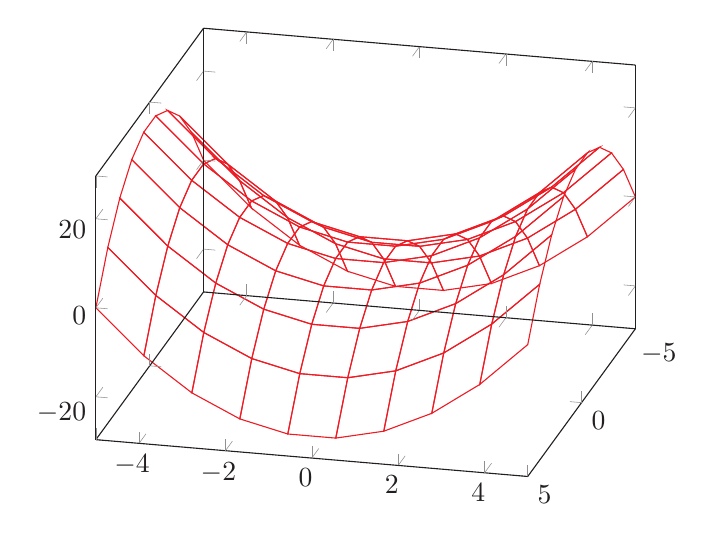
\begin{tikzpicture}
\begin{axis}[view/az=14]
    \addplot3 [
        mesh,
        draw=red,
        samples=10,
    ] {x^2-y^2};
\end{axis}
\end{tikzpicture}
\end{codeexample}

    Mesh plots use the |mesh legend| style to typeset legend images.
\end{plottype}

\begin{pgfplotskey}{mesh/check=\mchoice{false,warning,error} (initially error)}
    Allows to configure whether an error is generated if |mesh/rows| $\times$
    |mesh/cols| does not equal the total number of coordinates.

    If you know exactly what you are doing, it may be useful to disable the
    check. If you are unsure, it is best to leave the initial setting.
\end{pgfplotskey}

\begin{pgfplotskey}{z buffer=\mchoice{%
        default,
        none,
        auto,
        sort,
        reverse x seq,
        reverse y seq,
        reverse xy seq%
    } (initially default)%
}
    This key allows to choose between different $z$ buffering strategies. A $z$
    buffer determines which parts of an image should be drawn in front of other
    parts. Since both, the graphics packages \PGF{} and the final document
    format |.pdf| are inherently two dimensional, this work has to be done in
    \TeX{}. Currently, several (fast) heuristics can be used which work
    reasonably well for simple mesh and surface plots. Furthermore, there is a
    (time consuming) sorting method which also works if the fast heuristics
    fails.

    The $z$ buffering algorithms of \PGFPlots{} apply only to a single
    |\addplot| command. Different |\addplot| commands will be drawn on top of
    each other, in the order of appearance.

    The choice \declaretext{default} checks if we are currently working with a
    mesh or surface plot and uses |auto| in this case. If not, it sets
    |z buffer=none|.

    The choice \declaretext{none} disables $z$ buffering. This is also the case
    for two dimensional axes which don't need $z$ buffering.

    The choice \declaretext{auto} is the initial value for any mesh or surface
    plot: it uses a very fast heuristics to decide how to execute $z$ buffering
    for mesh and surface plots. The idea is to reverse either the sequence of
    all $x$-coordinates, or those of all $y$-coordinates, or both. For regular
    meshes, this suffices to provide $z$ buffering. In other words: the choice
    |auto| will use one of the three reverse strategies |reverse |*| seq| (or
    none at all). The choice |auto|, applied to |patch| plots, uses
    |z buffer=sort| since |patch| plots have no matrix structure.

    The choice \declaretext{sort} can be used for scatter, line, mesh, surface
    and patch plots. It sorts according to the depth of each point (or mesh
    segment). Sorting in \TeX{} uses a slow algorithm and may require a lot of
    memory (although it has the expected runtime asymptotics $\mathcal O(N \log
    N)$). The depth of a mesh segment is just \emph{one} number, currently
    determined as \emph{mean} over the vertex depths. Since |z buffer=sort| is
    actually just a more intelligent way of drawing mesh segments on top of
    each other, it may still fail. Failure can occur if mesh segments are large
    and overlap at different parts of the segment (see Wikipedia ``Painter's
    algorithm''). If you experience problems of this sort, consider reducing
    the mesh width (the mesh element size) such that they can be sorted
    independently (for example automatically using |patch refines=2|, see the
    |patchplots| library).

    The remaining choices apply only to mesh/surface plots (i.e.\@ for matrix
    data) and do nothing more then their name indicates: they reverse the
    coordinate sequences of the input matrix (using quasi linear runtime). They
    should only be used in conjunction by |z buffer=auto|.
\end{pgfplotskey}


\subsection{Surface Plots}
\label{sec:pgfplots:surfplots}

\begin{plottype}[/pgfplots]{surf}
    A surface plot visualizes a two dimensional, single patch using different
    fill colors for each patch segment. Each patch segment is a (pseudo)
    rectangle, that means input data is given in form of a data matrix as is
    discussed in the introductory Section~\ref{pgfplots:sec:threedim} about
    three dimensional coordinates.

\pgfplotsexpensiveexample
\begin{codeexample}[]
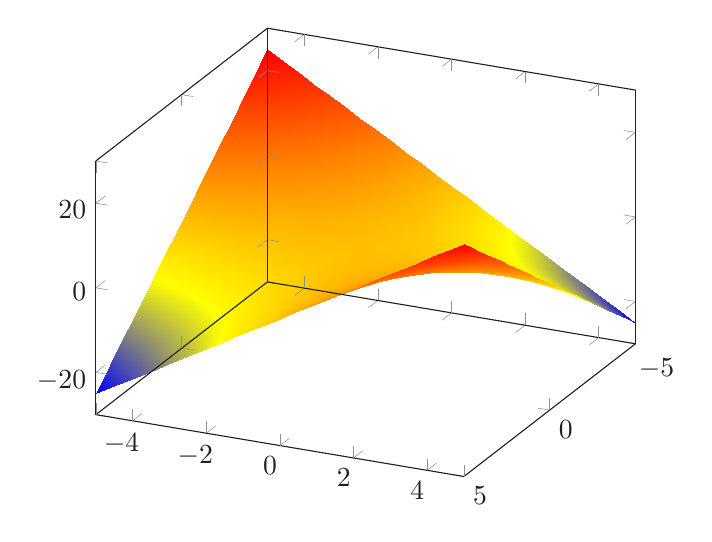
\begin{tikzpicture}
\begin{axis}
    \addplot3 [
        surf,
        shader=interp,
    ] {x*y};
\end{axis}
\end{tikzpicture}
\end{codeexample}

    The simplest way to generate surface plots is to use the plot expression
    feature, but -- as discussed in Section~\ref{pgfplots:sec:threedim} --
    other input methods like \verbpdfref{\addplot3 table} or
    \verbpdfref{\addplot3 coordinates} are also possible.

    The appearance can be configured using |colormap|s, the value of the
    |shader|, |faceted color| keys and the current |color| and/or |draw|/|fill|
    color. As for |mesh| plots, the special |color=mapped color| is installed
    for the faces. The stroking color for faceted plots can be set with
    |faceted color| (see below for details).

\pgfplotsexpensiveexample
\begin{codeexample}[]
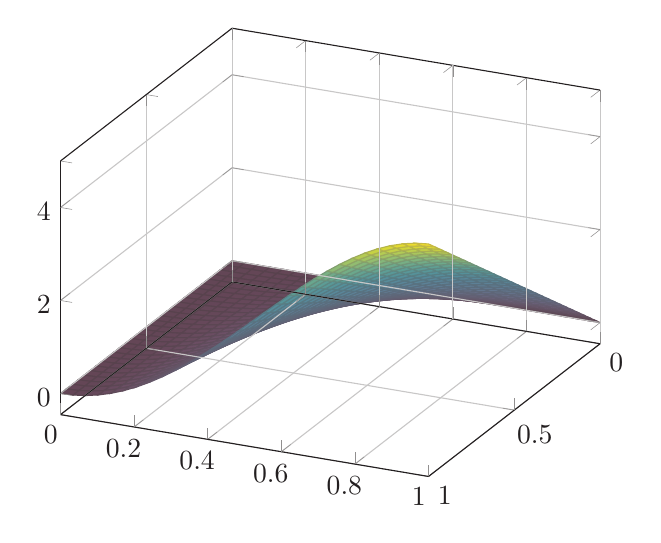
\begin{tikzpicture}
\begin{axis}[
    grid=major,
    colormap/viridis,
]
    \addplot3 [
        surf,
        samples=30,
        domain=0:1,
    ] {5*x*sin(2*deg(x)) * y};
\end{axis}
\end{tikzpicture}
\end{codeexample}

\pgfplotsexpensiveexample
\begin{codeexample}[]
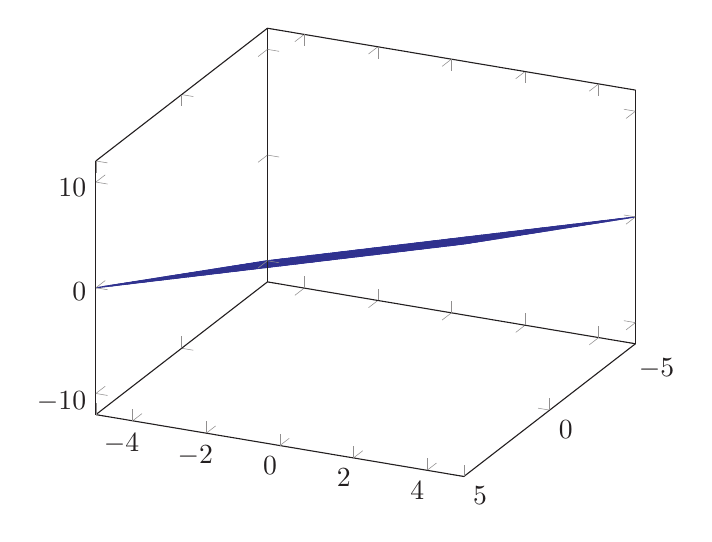
\begin{tikzpicture}
\begin{axis}
    \addplot3 [
        surf,
        faceted color=blue,
    ] {x+y};
\end{axis}
\end{tikzpicture}
\end{codeexample}

\pgfplotsexpensiveexample
\begin{codeexample}[]
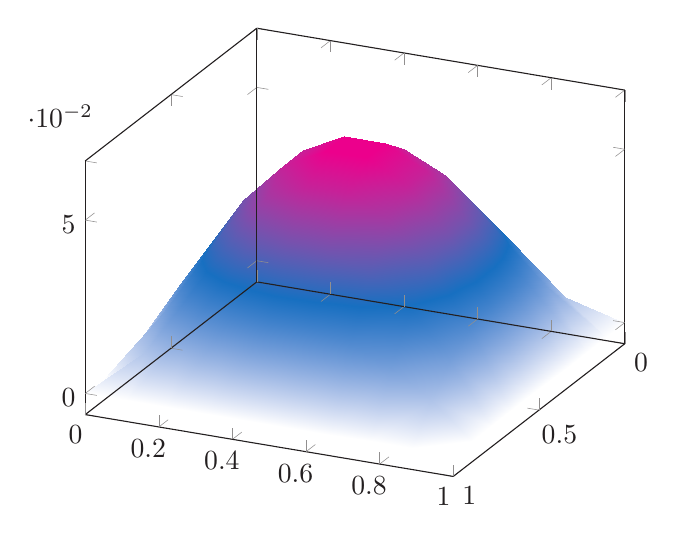
\begin{tikzpicture}
    \begin{axis}[colormap/cool]
        \addplot3 [surf,samples=10,domain=0:1,shader=interp]
            {x*(1-x)*y*(1-y)};
    \end{axis}
\end{tikzpicture}
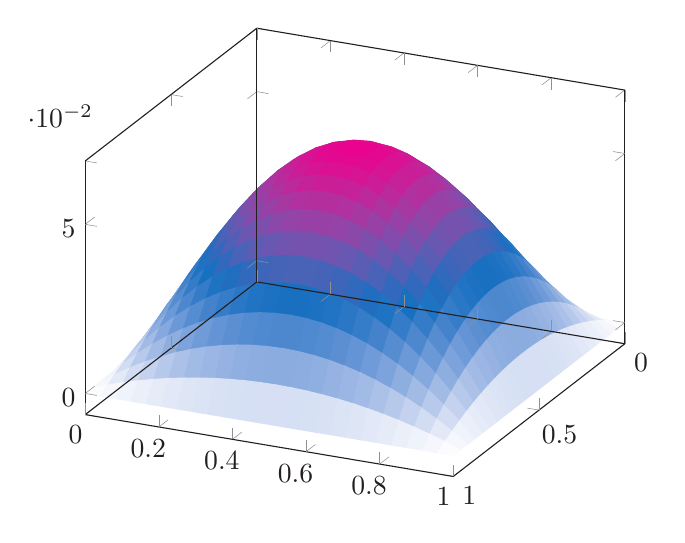
\begin{tikzpicture}
    \begin{axis}[colormap/cool]
        \addplot3 [surf,samples=25,domain=0:1,shader=flat]
            {x*(1-x)*y*(1-y)};
    \end{axis}
\end{tikzpicture}
\end{codeexample}

\pgfplotsexpensiveexample
\begin{codeexample}[]
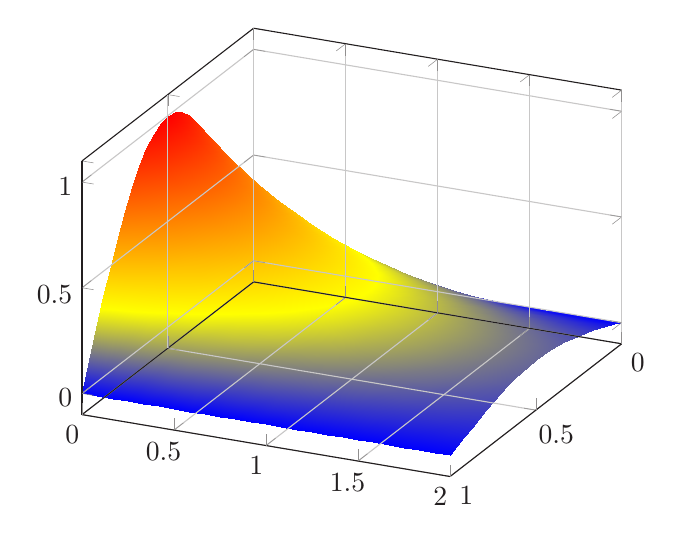
\begin{tikzpicture}
\begin{axis}[grid=major]
    \addplot3 [
        surf,
        shader=interp,
        samples=25,
        domain=0:2,
        y domain=0:1,
    ] {exp(-x) * sin(pi*deg(y))};
\end{axis}
\end{tikzpicture}
\end{codeexample}

\pgfplotsexpensiveexample
\begin{codeexample}[]
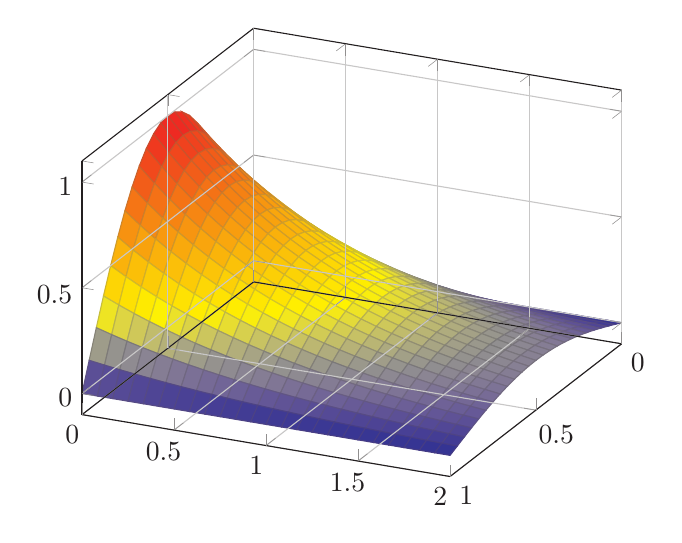
\begin{tikzpicture}
\begin{axis}[grid=major]
    \addplot3 [
        surf,
        shader=faceted,
        samples=25,
        domain=0:2,
        y domain=0:1,
    ] {exp(-x) * sin(pi*deg(y))};
\end{axis}
\end{tikzpicture}
\end{codeexample}

    Details about the shading algorithm are provided below in the documentation
    of |shader|.

    Surface plots use the |mesh legend| style to create legend images.
\end{plottype}

\begin{pgfplotskey}{shader=\mchoice{%
        flat,
        interp,
        faceted,
        flat corner,
        flat mean,
        faceted interp%
    } (initially faceted)%
}
    Configures the shader used for surface plots. The shader determines how the
    color data available at each single vertex is used to fill the surface
    patch.

    The simplest choice is to use one fill color for each segment, the choice
    \declareandlabel{flat}.

\pgfplotsexpensiveexample
\begin{codeexample}[]
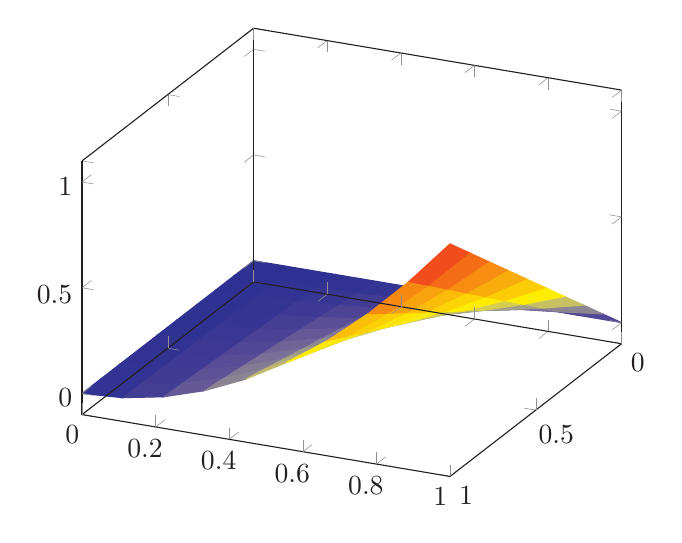
\begin{tikzpicture}
\begin{axis}
    \addplot3 [
        surf,
        shader=flat,
        samples=10,
        domain=0:1,
    ] {x^2*y};
\end{axis}
\end{tikzpicture}
\end{codeexample}

    \noindent There are (currently) two possibilities to determine the single
    color for every segment:
    %
    \begin{description}
        \item[\declaretext{flat corner}] Uses the color data of one vertex to
            color the segment. The color of the \emph{first} vertex
            determines the color of the entire segment. Note that \PGFPlots{}
            ensures that the outcome is always the same, even if the vertices
            are reordered due to |z buffer|ing or |mesh/ordering|.

            Note that \PGFPlots{} versions up to and including~1.12 chose one
            of them without respectiving reordering. In order to have the
            ordering independent of other features, you have to write
            |compat=1.13| or newer.
        \item[\declaretext{flat mean}] Uses the mean of all four color data
            values as segment color. This is the initial value as it provides
            symmetric colors for symmetric functions.
    \end{description}
    %
    The choice |flat| is actually the same as |flat mean|. Please note that
    |shader=flat mean| and |shader=flat corner| also influence mesh plots --
    the choices determine the mesh segment color.

    Another choice is |shader=|\declareandlabel{interp} which uses Goraud
    shading (smooth linear interpolation of two triangles approximating
    rectangles) to fill the segments.

\pgfplotsexpensiveexample
\begin{codeexample}[]
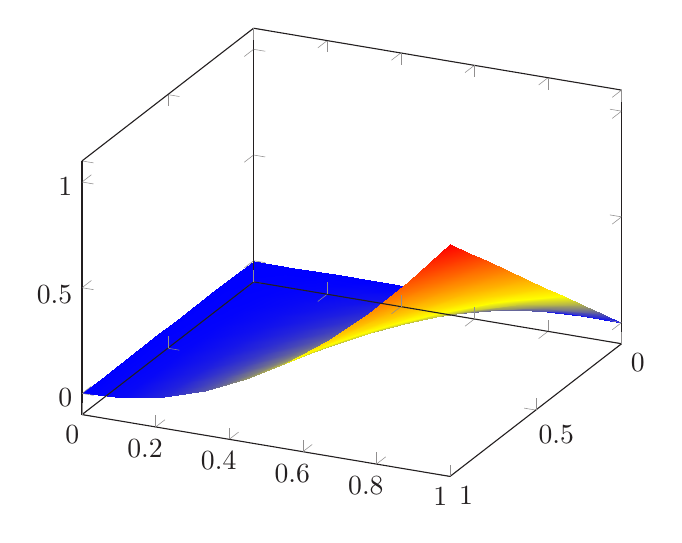
\begin{tikzpicture}
\begin{axis}
    \addplot3 [
        surf,
        shader=interp,
        samples=10,
        domain=0:1,
    ] {x^2*y};
\end{axis}
\end{tikzpicture}
\end{codeexample}

    The |shader=interp| employs a low-level shading implementation which is
    currently available for the following drivers:
    %
    \begin{itemize}
        \item the postscript driver |\def\pgfsysdriver{pgfsys-dvips.def}|,
        \item the |pdflatex| driver |\def\pgfsysdriver{pgfsys-pdftex.def}|,
        \item the |lualatex| driver |\def\pgfsysdriver{pgfsys-pdftex.def}| and \\
            |\def\pgfsysdriver{pgfsys-luatex.def}|,
        \item the |dvipdfmx| driver |\def\pgfsysdriver{pgfsys-dvipdfmx.def}|.
    \end{itemize}
    %
    For other drivers, the choice |shader=interp| will result in a warning and
    is equivalent to |shader=flat mean|. See also below for detail remarks.

    Note that |shader=interp,patch type=bilinear| allows real bilinear
    interpolation, see the |patchplots| library.

    The choice |shader=|\declareandlabel{faceted} uses a constant fill color
    for every mesh segment (as for |flat|) and the value of the key
    |/pgfplots/faceted color| to draw the connecting mesh elements:
    %
\pgfplotsexpensiveexample
\begin{codeexample}[]
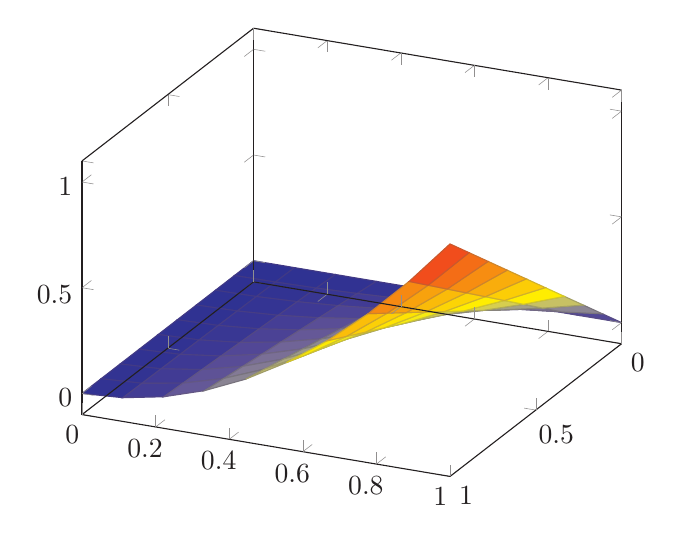
\begin{tikzpicture}
\begin{axis}
    \addplot3 [
        surf,
        shader=faceted,
        samples=10,
        domain=0:1,
    ] {x^2*y};
\end{axis}
\end{tikzpicture}
\end{codeexample}

    The last choice is |shader=|\declareandlabel{faceted interp}. As the name
    suggests, it is a mixture of |interp| and |faceted| in the sense that each
    element is shaded using linear triangle interpolation (see also the
    |patchplots| library for bilinear interpolation) in the same way as for
    |interp|, but additionally, the edges are colored in |faceted color|:
    %
\pgfplotsexpensiveexample
\begin{codeexample}[]
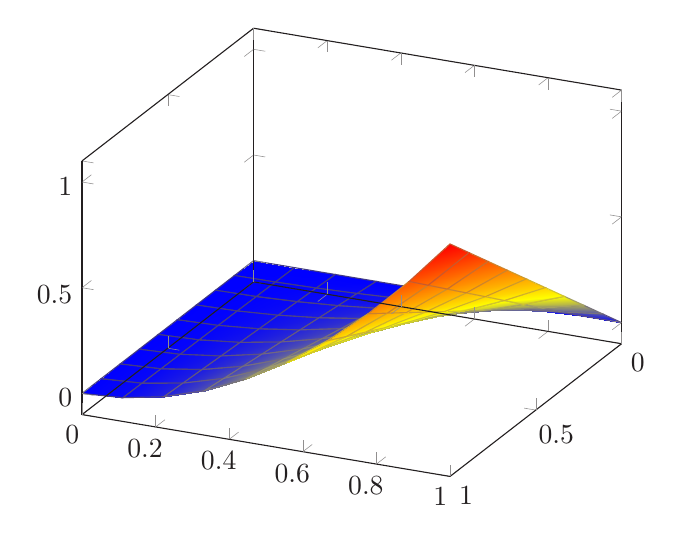
\begin{tikzpicture}
\begin{axis}
    \addplot3 [
        surf,
        shader=faceted interp,
        samples=10,
        domain=0:1,
    ] {x^2*y};
\end{axis}
\end{tikzpicture}
\end{codeexample}
    %
    \noindent In principle, there is nothing wrong with the idea as such, and
    it looks quite good -- but it enlarges the resulting PDF document
    considerably and might take a long time to render. It works as follows: for
    every mesh element (either triangle for |patch| plots or rectangle for
    lattice plots), it creates a low level shading. It then fills the single
    mesh element with that shading, and strokes the edges with |faceted color|.
    The declaration of that many low level shadings is rather inefficient in
    terms of PDF objects (large output files) and might render
    slowly.\footnote{My experience is as follows: Acrobat reader can efficiently
    render huge \texttt{interp} shadings. But it is very slow for
    \texttt{faceted interp} shadings. Linux viewers like xpdf are reasonably
    efficient for \texttt{interp} (at least with my bugfixes to libpoppler) and
    are also fast for \texttt{faceted interp} shadings.} For orthogonal plots
    (like |view={0}{90}|), the effect of |faceted interp| can be gained with
    less cost if one uses two separate |\addplot| commands: one with |surf| and
    one with |mesh|. Handle this choice with care.


    \paragraph{Details:}

    \begin{itemize}
        \item All shaders support |z buffer=sort| (starting with version
            1.4).
        \item The choice |shader=faceted| is the same as |shader=flat| --
            except that it uses a special draw color.

            So, |shader=faceted| has the same effect as

            |shader=flat,draw=\pgfkeysvalueof{/pgfplots/faceted color}|.
        \item The |flat| shader uses the current |draw| and |fill| colors.
            They are set with |color=mapped color| and can be overruled with
            |draw=|\meta{draw color} and |fill=|\meta{fill color}. The
            |mapped color| always contains the color of the color map.
        \item You easily add |mark=|\meta{plot mark} to mesh and/or surface
            plots or even colored plot marks with |scatter|. The scatter plot
            feature will use the same color data as for the surface.

            But: Markers and surfaces do not share the same depth
            information. They are drawn on top of each other.
        \item Remarks on |shader=interp|:
            %
            \begin{itemize}
                \item It uses the current color map in any case, ignoring
                    |draw| and |fill|.
                \item For surface plots with lots of points,
                    |shader=interp| produces smaller |pdf| documents,
                    requires less compilation time in \TeX{} and requires
                    less time to display in Acrobat Reader than
                    |shader=flat|.
                \item The postscript driver \emph{truncates} coordinates to
                    24~bit -- which might result in a loss of precision
                    (the truncation is not very intelligent). See the
                    |surf shading/precision| key for details. To improve
                    compatibility, this 24 bit truncation algorithm is enabled
                    by default also for PDF documents.
                \item The choice |shader=interp| works well with either
                    Acrobat Reader or recent versions of free
                    viewers.\footnote{The author of this package has
                    submitted bugfixes to xpdf/libpoppler which should be
                    part of the current stable versions of many viewers.}
                    However, some free viewers show colors incorrectly
                    (like evince). I hope this message will soon become
                    outdated\ldots{} if not, provide bug reports to the
                    Linux community to communicate the need to improve
                    support for Type 4 (|patch|) and Type 5 PDF (|surf|)
                    and Type 7 (|patch| and elements of the |patchplots|
                    library) shadings.
                \item The |interp| shader yields the same outcome as
                    |faceted interp,faceted color=none|, although
                    |faceted interp| requires much more resources.
            \end{itemize}
    \end{itemize}

\pgfplotsexpensiveexample
\begin{codeexample}[]
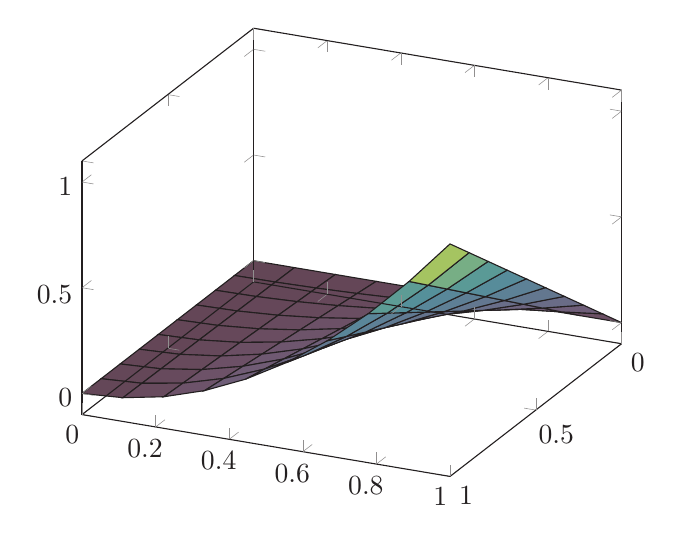
\begin{tikzpicture}
\begin{axis}[colormap/viridis]
    \addplot3 [
        surf,
        shader=flat,
        draw=black,
        samples=10,
        domain=0:1,
    ] {x^2*y};
\end{axis}
\end{tikzpicture}
\end{codeexample}

\pgfplotsexpensiveexample
\begin{codeexample}[]
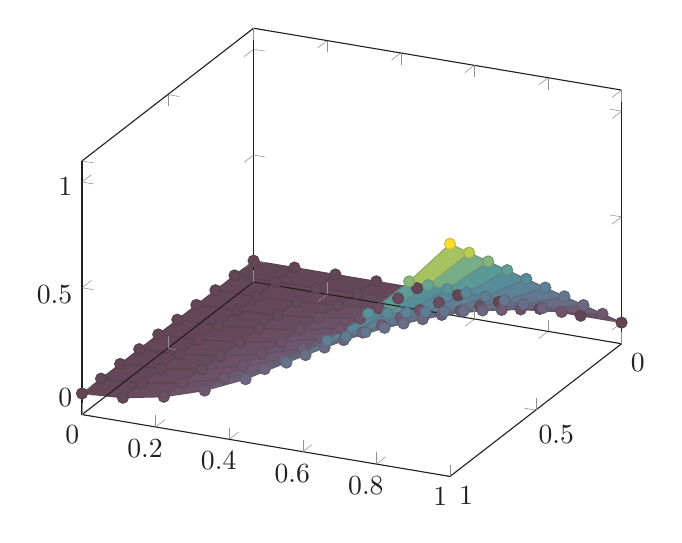
\begin{tikzpicture}
\begin{axis}[colormap/viridis]
    \addplot3 [
        surf,
        shader=faceted,
        scatter,mark=*,
        samples=10,
        domain=0:1,
    ] {x^2*y};
\end{axis}
\end{tikzpicture}
\end{codeexample}

    Note that the |shader| always interacts with |colormap access|. In
    particular, |colormap access=piecewise constant| combined with
    |shader=interp| results in a filled contour plot, see
    Section~\ref{sec:pgfplots:filled:contour} for details.
\end{pgfplotskey}

\begin{pgfplotskey}{faceted color=\marg{color name} (initially mapped color!80!black)}
    Defines the color to be used for meshes of faceted surface plots.

    Set |faceted color=none| to disable edge colors.
\end{pgfplotskey}

{
\tikzset{
    external/figure name/.add={}{interior_colormap_},
    /pdflinks/search key prefixes in/.add={}{,/pgfplots/mesh/},
}%
\begin{pgfplotskeylist}{%
    mesh/interior colormap=\marg{map name}\marg{colormap specification},%
    mesh/interior colormap name=\marg{map name}%
}
    Allows to use a different |colormap| for the ``other side'' of the surface.

    Each mesh has two sides: one which ``points'' to the view's origin and one
    which points away from it. This key allows to define a second |colormap|
    for the side which points away from the view's origin. The motivation is to
    distinguish between the outer side and the interior parts of a surface:
    %
\pgfplotsexpensiveexample
\begin{codeexample}[]
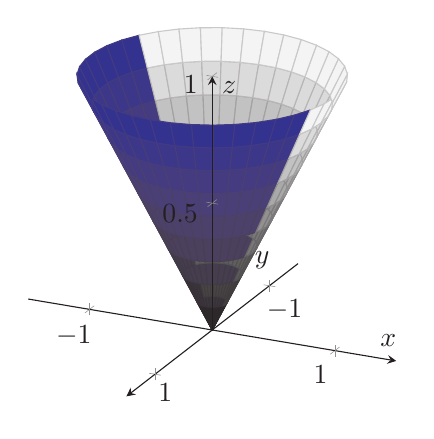
\begin{tikzpicture}
\begin{axis}[
    axis lines=center,
    axis on top,
    xlabel={$x$}, ylabel={$y$}, zlabel={$z$},
    domain=0:1,
    y domain=0:2*pi,
    xmin=-1.5, xmax=1.5,
    ymin=-1.5, ymax=1.5, zmin=0.0,
    mesh/interior colormap=
        {blueblack}{color=(black) color=(blue)},
    colormap/blackwhite,
    samples=10,
    samples y=40,
    z buffer=sort,
]
    \addplot3 [surf]
        ({x*cos(deg(y))},{x*sin(deg(y))},{x});
\end{axis}
\end{tikzpicture}
\end{codeexample}

    \noindent The |interior colormap| is often the one for the ``inner side''.
    However, the orientation of the surface depends on its normal vectors:
    \PGFPlots{} computes them using the right-hand-rule. The right-hand-rule
    applied to a triangle means to take the first encountered point, point the
    thumb in direction of the second point and the first finger in direction of
    the third point. Then, the normal for that triangle is the third finger
    (i.e.\@ the cross product of the involved oriented edges). For rectangular
    patches, \PGFPlots{} uses the normal of one of its triangles.\footnote{This
    may change in future versions.} Consequently, |mesh/interior colormap|
    will only work if the involved patch segments are consistently oriented.

    A patch whose normal vector points into the same direction as the view
    direction uses the standard |colormap name|. A patch whose normal vector
    points into the opposite direction (i.e.\@ in direction of the viewport)
    uses |mesh/interior colormap|.

\pgfplotsexpensiveexample
\begin{codeexample}[]
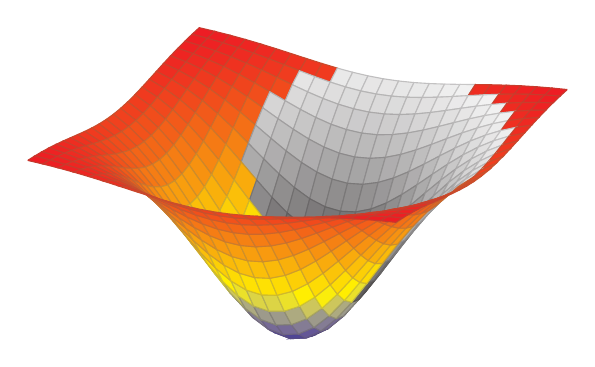
\begin{tikzpicture}
\begin{axis}[
    hide axis,
    xlabel=$x$,ylabel=$y$,
    mesh/interior colormap name=hot,
    colormap/blackwhite,
]
    \addplot3 [domain=-1.5:1.5,surf]
        {-exp(-x^2-y^2)};
\end{axis}
\end{tikzpicture}
\end{codeexample}

    The implementation of |mesh/interior colormap| works well for most
    examples; in particular, if the number of samples is large enough to
    resolve the boundary between inner and outer colormap. However, it might
    still produce spurious artifacts:
    %
\pgfplotsexpensiveexample
\begin{codeexample}[]
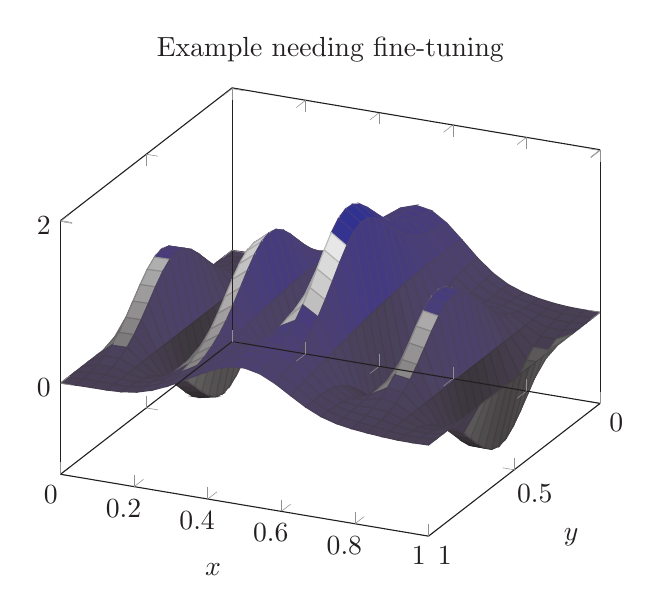
\begin{tikzpicture}
\begin{axis}[
    title=Example needing fine-tuning,
    xlabel=$x$,
    ylabel=$y$,
]
    \addplot3 [surf,
        mesh/interior colormap={blueblack}{
            color=(black) color=(blue)
        },
        colormap/blackwhite,
        domain=0:1,
    ] {
        sin(deg(8*pi*x))* exp(-20*(y-0.5)^2)
            + exp(-(x-0.5)^2*30
                - (y-0.25)^2 - (x-0.5)*(y-0.25))
    };
\end{axis}
\end{tikzpicture}
\end{codeexample}
    %
    \noindent The previous example has need for improvement with respect to a
    couple of aspects: first, it has small overshoots near some of the meshes
    vertices (especially on top of the hills). These can be fixed using
    |miter limit=1|. Second, the boundary between blue and black is incorrect.
    This can be improved by means of an increased sampling density
    (|samples=31|). In addition, we can configure \PGFPlots{} to move the
    boundary between the two colormaps in favor of the blue region using
    |mesh/interior colormap thresh| as follows:
    %
\pgfplotsexpensiveexample
\begin{codeexample}[]
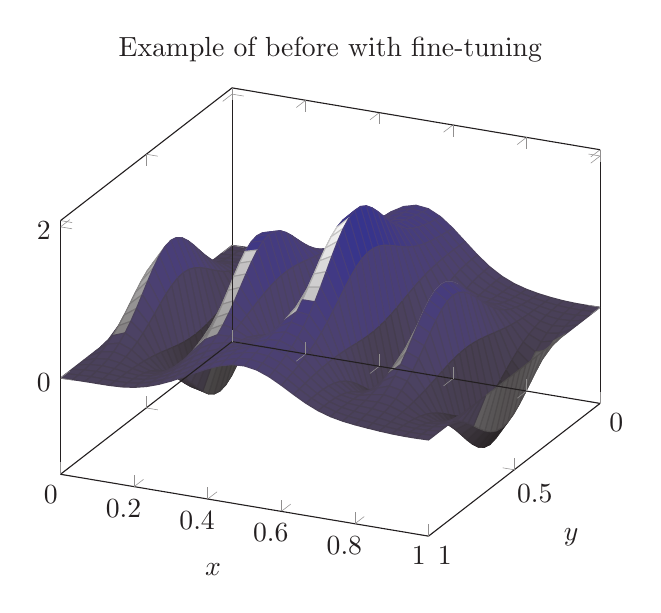
\begin{tikzpicture}
\begin{axis}[
    title=Example of before with fine-tuning,
    xlabel=$x$,
    ylabel=$y$,
]
    \addplot3 [
        surf,
        mesh/interior colormap={blueblack}{
            color=(black) color=(blue)
        },
        % slightly increase sampling quality (was 25):
        samples=31,
        % avoids overshooting corners:
        miter limit=1,
        % move boundary between inner and outer:
        mesh/interior colormap thresh=0.1,
        colormap/blackwhite,
        domain=0:1,
    ] {
        sin(deg(8*pi*x))* exp(-20*(y-0.5)^2)
            + exp(-(x-0.5)^2*30
                - (y-0.25)^2 - (x-0.5)*(y-0.25))
    };
\end{axis}
\end{tikzpicture}
\end{codeexample}
    %
    \noindent This improves the display.


    \paragraph{Call for volunteers:}

    it would be nice if the fine-tuning of these keys would be unnecessary. If
    someone has well-founded suggestions (like knowledge and perhaps exhaustive
    experiments) on how to improve the feature, let me know.

    Note that |mesh/interior colormap| cannot be combined with |mesh/refines|
    currently.

    Note that |mesh/interior colormap| will increase compilation times due to
    the computation of normal vectors.
\end{pgfplotskeylist}

\begin{pgfplotskey}{mesh/interior colormap thresh=\marg{Number between $-1.0$ and $+1.0$} (initially 0)}
    A threshold which moves the boundary between the |colormap| and
    |interior colormap| in favor of |colormap| (if the value is negative) or in
    favor of |interior colormap| (if the value is positive).

    The extreme value $-1$ essentially deactivates |interior colormap| whereas
    the other extreme $+1$ deactivates |colormap|.

    See above for an example.
\end{pgfplotskey}
}

\begin{pgfplotskey}{surf shading/precision=\mchoice{pdf,postscript,ps} (initially postscript)}
    A key to configure how the low level driver for |shader=interp| writes its
    data. The choice |pdf| uses 32~bit binary coordinates (which is lossless).
    The resulting |.pdf| files appear to be correct, but they can't be
    converted to postscript -- the converter software always complains about an
    error.

    The choice |postscript| (or, in short, |ps|) uses 24~bit truncated binary
    coordinates. This results in both, readable |.ps| and |.pdf| files.
    However, the truncation is lossy.

    If anyone has ideas how to fix this problem: let me know. As far as I know,
    Postscript should accept 32~bit coordinates, so it might be a mistake in
    the shading driver.
\end{pgfplotskey}


\subsection{Surface Plots with Explicit Color}

{
\tikzset{
    external/figure name/.add={}{surf_explicit_color_},
    /pdflinks/search key prefixes in/.add={}{,/pgfplots/mesh/},
}

The surface plots described in Section~\ref{sec:pgfplots:surfplots} are all
based on |colormap|s. This section introduces a different type of surface plot.
In fact, it uses the very same plot handlers: it applies to |mesh|, |surf|, and
|patch| plots. However, the way colors are provided and the way \PGFPlots{}
interpolates colors is substantially different.

This section describes surface plots with explicit colors. These expect colors
like |red|, |green|, or |rgb=(0.5,0.2,1)| for every vertex of the |mesh| -- and
interpolates smoothly between these vertices. This appears to be simpler,
perhaps even more straightforward than |surf|ace plots based on |colormap|s. It
is not. Surface plots with explicit color are more difficult to define, and
they are more difficult to read.

If you are in doubt of whether to use a surface colored by a |colormap| or
explicit colors, you should prefer |colormap|s for reasons discussed below.

\begin{pgfplotskey}{mesh/color input=\mchoice{colormap,explicit,explicit mathparse} (initially colormap)}
    Allows to configure how \PGFPlots{} expects color input for surface plots.

    The choice \declaretext{colormap} uses the standard colormaps. This
    particular choice expects scalar values of |point meta| which are mapped
    linearly into the colormap. It resembles the surface plots which are
    explained in more detail in Section~\ref{sec:pgfplots:surfplots}. It is the
    default configuration and covers (probably) most common use cases.

    The choice \declaretext{explicit} expects explicitly provided |point meta|
    of symbolic form: every coordinate of your input coordinate stream is
    supposed to have an explicitly defined color as |point meta|. Here,
    ``explicitly provided'' refers to |point meta=explicit symbolic|. This
    choice and the available color formats are explained in all detail in the
    following subsections.
    % (more precisely: in Section~\ref{sec:surf:explicit:color}).

    The choice \declaretext{explicit mathparse} is similar to |explicit|, but
    it allows to provide just one math expression which is evaluated for every
    coordinate. The math expression can be of the form |rgb=x,y,0.5| in which
    case |x| is used to define the ``red'' component, |y| is used to define the
    ``green'' component and the ``blue'' component is fixed to |0.5|. This key
    is also explained in more detail in the following subsections.
    %, especially in Section~\ref{sec:surf:explicit:color:math}.
\end{pgfplotskey}

The main use case of |mesh/color input=|\declaretext{colormap} is to allow a
map between the interpolated colors and some value of interest. This map can be
shown as |colorbar|:
%
% \usepgfplotslibrary{patchplots}
\begin{codeexample}[]
% \usepgfplotslibrary{patchplots}
\begin{tikzpicture}
\begin{axis}[small,view={0}{90},colorbar]
    \addplot3 [
        surf,
        shader=interp,
        patch type=bilinear,
    ] coordinates {
        (0,0,0) (1,0,0)

        (0,1,0) (1,1,1)
    };
\end{axis}
\end{tikzpicture}
\end{codeexample}
%
\noindent Note that the preceding example is a standard |surf| plot except for
|patch type=bilinear| which controls how color is to be interpolated. There is
a $2 \times 2$ matrix, and its $z$ values are used as color data. Clearly,
value $z=0$ corresponds to blue and $z=1$ corresponds to red -- and all other
colors in-between are not directly related to blue and red; they are taken from
the colormap. The colormap defines which colors appear: those which make up the
colormap and those which can occur as interpolated colors between the colors of
the color map. The pairwise mixture of colors is a property of
|mesh/color input=colormap|, not of |mesh/color input=explicit| (where more
than two colors are mixed together). Furthermore, the surface indicates
contours of constant $z$ level. Take, for example, the yellow contour. We know
that it has some value between $0.3$ and $0.4$, say $0.35$. Since these
shadings are continuous, we know that the point $z=0.35$ occurs between $z=0$
and $z=1$ -- at every point of the surface. Due to the colormap, each point on
the surface which has $z=0.35$ will receive the yellow color. This is because
the interpolation is carried out on the scalar |point meta| value, which is
afterwards mapped into the |colormap|. This contour property is also unique for
colormap surfaces.

The other two choices are explained in all detail in the next subsections.


\subsubsection{Providing Colors Explicitly For Each Coordinate}
\label{sec:surf:explicit:color}

Here is a simple approach with the same vertices as the colormap example above,
but with explicit colors:
%
% \usepgfplotslibrary{patchplots}
\begin{codeexample}[]
% \usepgfplotslibrary{patchplots}
\begin{tikzpicture}
\begin{axis}[small,view={0}{90}]
    \addplot3 [
        surf,
        shader=interp,
        patch type=bilinear,
        mesh/color input=explicit,
    ] coordinates {
        (0,0,0) [color=blue]   (1,0,0) [color=green]

        (0,1,0) [color=yellow] (1,1,1) [color=red]
    };
\end{axis}
\end{tikzpicture}
\end{codeexample}
%
\noindent The coordinates and the view is the same, even the way colors are
being interpolated bilinearly. However, we have four different colors in the
corners. We see these corners in the output, and we see that they are smoothly
mixed together. However, the mix contains all four colors, not just two. As a
direct consequence, there are no contour lines.

The absence of direct information how to map color information to ``some
information of the data visualization'' implies that \emph{if} you want to use
|surf|ace plots with explicit color, you have to state clearly what you want to
show. This is considerably simpler for |colormap|s.

The following example configures $z=0$ to receive |blue| and $z=1$ to receive
|red| as in our preceding |colormap| example (see above) using
|mesh/color input=|\declaretext{explicit}.
%
% \usepgfplotslibrary{patchplots}
\begin{codeexample}[]
% \usepgfplotslibrary{patchplots}
\begin{tikzpicture}
\begin{axis}[small,view={0}{90}]
    \addplot3 [
        surf,
        shader=interp,
        patch type=bilinear,
        mesh/color input=explicit,
    ] coordinates {
        (0,0,0) [color=blue] (1,0,0) [color=blue]

        (0,1,0) [color=blue] (1,1,1) [color=red]
    };
\end{axis}
\end{tikzpicture}
\end{codeexample}
%
\noindent We see the bilinear nature of the interpolation; it is related to
that of |mesh/color input=colormap| above (compare the contour lines
in-between). In most cases, you simply want to show some contour lines. And for
such cases, a |colormap| is the way to go.

There might be cases where |mesh/color input=explicit| is adequate. However,
you will need to think it through properly. And you need to explain clearly
what you did because your audience will also have to think a lot before they
make sense of any data visualization based on explicit color interpolation.

The choice |mesh/color input=explicit| expects a choice of |point meta| which
results in symbolic values. In this context, ``symbolic'' refers to a special
color definition:
%
\begin{codeexample}[]
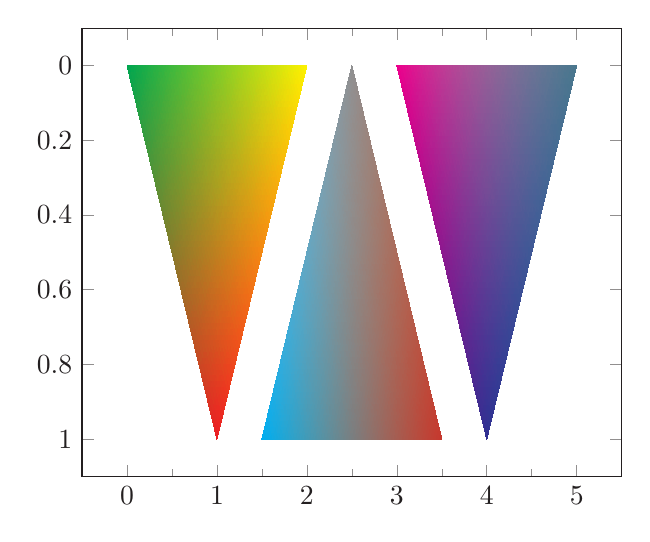
\begin{tikzpicture}
\begin{axis}[minor x tick num=1]
    \addplot [
        patch,
        shader=interp,
        mesh/color input=explicit,
    ] table [meta=c] {
        x y c
        0 0 color=green
    % default color model is rgb:
        1 1 1,0,0
        2 0 1,1,0

        1.5 1 cmyk=1,0,0,0
        2.5 0 gray=0.5
        3.5 1 color=red!80!black

        3 0 1,0,1
        4 1 0,0,1
        5 0 rgb255=0,128,128
    };
\end{axis}
\end{tikzpicture}
\end{codeexample}
%
\noindent The previous example defines a |patch| plot with three triangle
patches, each made up of three vertices which are placed as is into the input
coordinate stream. Each vertex has its color data in column~|c|. The format of
color specifications is explained in more detail in the following paragraph.

As soon as you write |mesh/color input=explicit|, \PGFPlots{} checks the
current value of |point meta|. If the current value of |point meta| is |none|,
it is set to |point meta=explicit symbolic| (that is what happened in our
example above). If the current value of |point meta| is some choice which
yields numeric output (like |point meta=x| or |point meta=\thisrow{x}+1|), it
is set to |point meta=explicit symbolic|. If the current value of |point meta|
is already of symbolic form, it is left unchanged.

Consequently, our example above sets |point meta=explicit symbolic| as soon as
it encounters |mesh/color input=explicit|. The explicit symbolic input handler
in turn expects the coordinate stream to provide point meta data for every
streamed coordinate. We use a table here, and a table reads its color data from
the column name provided in the |table/meta| key.

The accepted format of colors is quite similar to that of colormap definitions
(compare Section~\ref{sec:colormap:input:format} on
page~\pageref{sec:colormap:input:format}). The common format is
\declaretext{\meta{color model}|=|\meta{arguments}}. In contrast to the similar
input format inside of colormap definitions, the syntax here has no round
braces and does not have the \meta{length} argument. Nevertheless, the same
\meta{color model}s with the same \meta{arguments} are accepted. The choices
are
%
% ATTENTION : a VERY similar description (actually: the same) is in the
% colormap section
% maintain both; the syntax is different
\begin{description}
        \renewcommand\makelabel[1]{\declaretext{#1}}%
        \setlength{\labelsep}{0pt}
    \item[rgb] |=|\meta{red}|,|\meta{green}|,|\meta{blue} where each
        component is in the interval $[0,1]$,
    \item[rgb255] |=|\meta{red}|,|\meta{green}|,|\meta{blue} is similar to
        |rgb| except that each component is expected in the interval
        |[0,255]|,
    \item[gray] |=|\meta{value} with \meta{value} in the interval $[0,1]$,
    \item[color] |=|\meta{named color} where \meta{named color} is a
        predefined (named) color like `|red|' or a color expression like
        `|red!50|',
    \item[cmyk]
        |=|\meta{cyan}|,|\meta{magenta}|,|\meta{yellow}|,|\meta{black} where
        each component is in the interval $[0,1]$,
    \item[cmyk255]
        |=|\meta{cyan}|,|\meta{magenta}|,|\meta{yellow}|,|\meta{black} is the
        same as |cmyk| but expects components in the interval $[0,255]$,
    \item[cmy] |=|\meta{cyan}|,|\meta{magenta}|,|\meta{yellow} where each
        component is in the interval $[0,1]$,
    \item[hsb] |=|\meta{hue}|,|\meta{saturation}|,|\meta{brightness} where
        each component is in the interval $[0,1]$,
    \item[Hsb] |=|\meta{hue}|,|\meta{saturation}|,|\meta{brightness} is the
        same as |hsb| except that \meta{hue} is accepted in the interval
        $[0,360]$ (degree),
    \item[HTML] |=|\meta{hex red}\meta{hex green}\meta{hex blue} where
        component is expected to be a hex number between |00| and |FF| (a
        variant of |rgb255|),
    \item[wave] |=|\meta{wave length} which expects a single wave length as
        numeric argument in the range $[363,814]$.
\end{description}


\begin{pgfplotskey}{mesh/colorspace explicit color input=\mchoice{%
        rgb,rgb255,
        cmy,
        cmyk,cmyk255,
        gray,
        wave,
        hsb\\,Hsb,
        HTML%
    } (initially rgb)%
}
    If the input color has \emph{no color model}, the color components are
    interpreted as color in the color model specified as argument to this key.

    This key has just one purpose: to omit the \meta{color model} if it is the
    same for lots of points anyway.
\end{pgfplotskey}

\begin{pgfplotskey}{%
    mesh/colorspace explicit color output=\mchoice{rgb,cmyk,gray} (initially rgb)%
}
    Any color which is encountered by the survey phase (i.e.\@ while inspecting
    the |point meta| value) is immediately transformed into the color space
    configured as |mesh/colorspace explicit color output|.

    Note that this option has \emph{no effect} if you told |xcolor| to override
    the color space globally. More precisely, the use of
    %
\begin{codeexample}[code only]
\usepackage[cmyk]{xcolor}
\end{codeexample}
    %
    or, alternatively,
    %
\begin{codeexample}[code only]
\selectcolormodel{cmyk}
\end{codeexample}
    will cause all colors to be converted to |cmyk|, and \PGFPlots{} honors
    this configuration. Consequently, both these statements cause all colors to
    be interpolated in the desired color space, and all output colors will use
    this colorspace. This is typically exactly what you need.

    The transformed color is used for any color interpolation. In most cases,
    this is done by the |shader|, but it applies to |patch refines| and
    |patch to triangles| as well.

    Because the transformed color is used for color interpolation, the list of
    available \emph{output} color spaces is considerably smaller than the
    available \emph{input} color spaces. Only the device color spaces
    \declaretext{rgb}, \declaretext{gray}, and \declaretext{cmyk} are available
    as value for |mesh/colorspace explicit color output|.

    Any necessary colorspace transformations rely on the |xcolor|
    package.\footnote{Colorspace transformations are unavailable for plain
    \TeX{} and Con\TeX{}t. For these cases, you have to ensure that input and
    output color model are the same.} Note that colorspace transformations are
    subject to nearest color matching, i.e.\@ they are less accurate. This is
    typically far beyond pure rounding issues; it is caused by the fact that
    these color spaces are actually so different that transformations are hard
    to accomplish. If you can specify colors immediately in the correct color
    space, you can eliminate such transformations.

    Here is the same shading, once with CMYK output and once with RGB output.
    Depending on your output media (screen or paper), you will observe slightly
    different colors when comparing the pictures.
    %
\begin{codeexample}[]
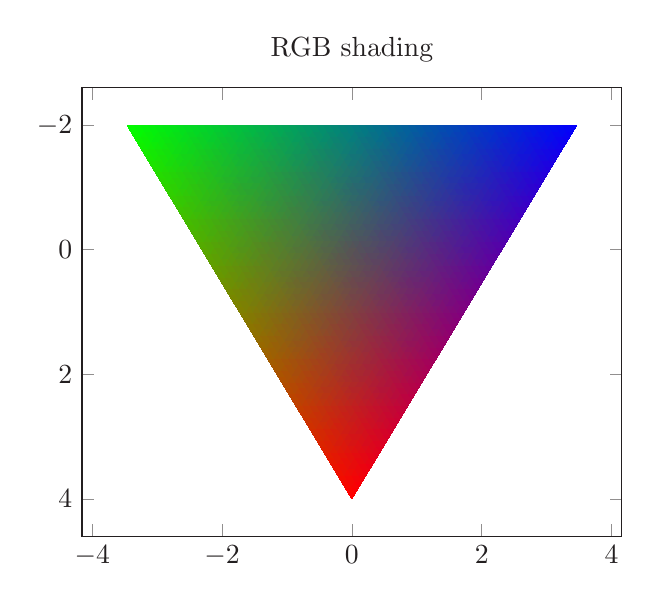
\begin{tikzpicture}
\begin{axis}[title=RGB shading]
    \addplot [
        patch,
        shader=interp,
        mesh/color input=explicit,
        mesh/colorspace explicit color output=rgb,
        data cs=polar,
    ] coordinates {
        (90,4)  [color=red]
        (210,4) [color=green]
        (-30,4) [color=blue]
    };
\end{axis}
\end{tikzpicture}
\end{codeexample}

\begin{codeexample}[]
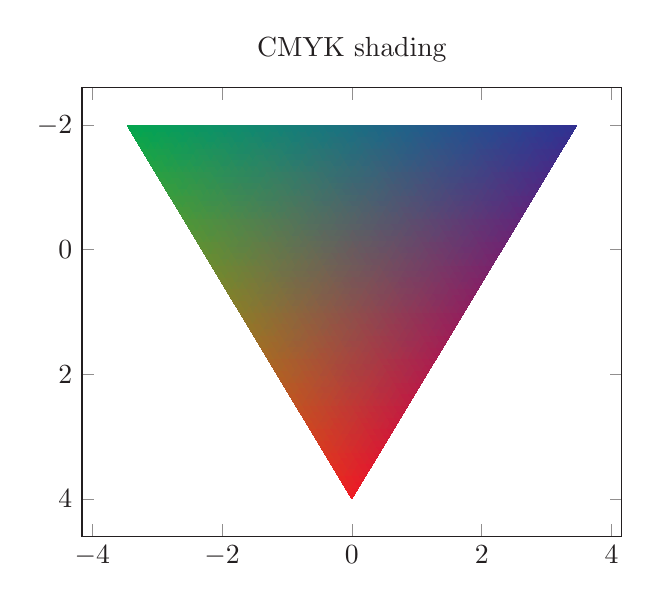
\begin{tikzpicture}
\begin{axis}[title=CMYK shading]
    \addplot [
        patch,
        shader=interp,
        mesh/color input=explicit,
        mesh/colorspace explicit color output=cmyk,
        data cs=polar,
    ]
    coordinates {
        (90,4)  [color=red]
        (210,4) [color=green]
        (-30,4) [color=blue]
    };
\end{axis}
\end{tikzpicture}
\end{codeexample}

    This key is similar to the related key |colormap default colorspace|,
    although the values can be chosen independently.
\end{pgfplotskey}


\subsubsection{Providing Color Components as Table}

The previous section shows how to provide a single symbolic color expression
for each coordinate, namely using |point meta=explicit symbolic|.

Another use case might be to provide a table containing both the coordinate
values and one column by color component. In order to assemble the color
specification from the input table, you can provide a symbolic expression:
%
\begin{codeexample}[]
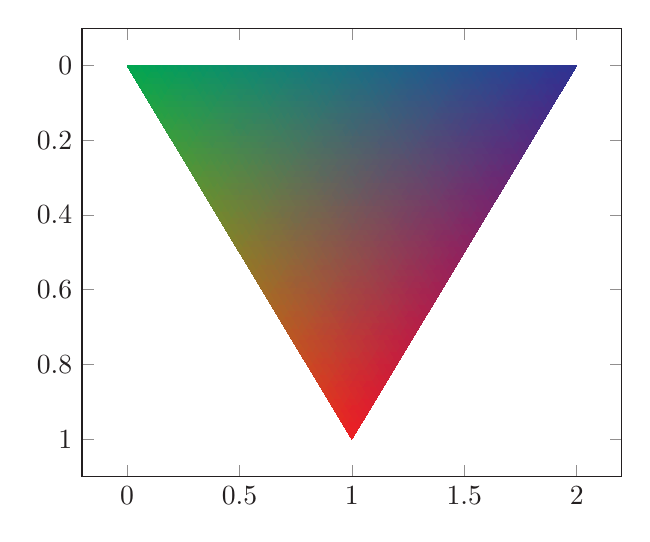
\begin{tikzpicture}
\begin{axis}
    \addplot [
        patch,
        shader=interp,
        mesh/color input=explicit,
        point meta={symbolic=
            {\thisrow{R},\thisrow{G},\thisrow{B}}
        },
    ] table {
        x y R G B
        0 0 0 1 0
        1 1 1 0 0
        2 0 0 0 1
    };
\end{axis}
\end{tikzpicture}
\end{codeexample}
%
The preceding example employs a |patch| plot with triangular elements as we
have seen before. Furthermore, it uses explicit color input -- but combined
with |point meta={symbolic=|\marg{value}|}| (note the extra pair of braces).
This choice accepts arbitrary symbols on input which will be reevaluated
(expanded) for every coordinate. In our example, we simply read the values from
table columns using |\thisrow|. Since the default input colorspace is RGB, this
results in the expected triangle with red, green, and blue corners. The result
has to form a valid color specification.

Note that the symbolic expression is purely string based in this context. If
you plan to use math expressions, you have to use
|mesh/color input=explicit mathparse| as explained in the following section.


\subsubsection{Providing Colors as Math Expression}
\label{sec:surf:explicit:color:math}

The key |mesh/color input| has two choices for explicit color input. The choice
\declaretext{explicit} has been discussed in the preceding paragraphs, it
expects one color specification for every node for which colors are needed. It
also accepts a kind of string based expressions to concatenate the expected
color specification in a suitable way.

The second choice |mesh/color input=|\declaretext{explicit mathparse} is almost
the same -- with one major difference: it allows to provide math expressions
inside of the |point meta| value. However, the provided math expressions need
to form a color specification which typically has more than one color
component.

With this choice, the value of |point meta| is of symbolic form, but the color
components are reevaluated with the math parser for every input point which has
color data. The most convenient way to provide such expressions is
|point meta={symbolic={|\meta{R},\meta{G},\meta{B}|}}| (again, note the extra
set of braces for the argument).

\begin{codeexample}[]
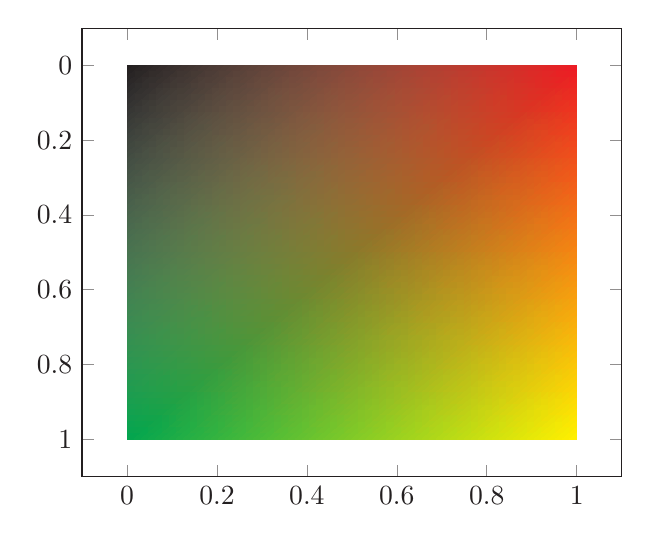
\begin{tikzpicture}
\begin{axis}
    \addplot [
        surf,
        shader=interp,
        mesh/color input=explicit mathparse,
        point meta={symbolic={x,\thisrow{y},0}},
    ] table {
        x y
        0 0
        1 0

        0 1
        1 1
    };
\end{axis}
\end{tikzpicture}
\end{codeexample}
%
\noindent The preceding example is a |surf|ace plot with a $2 \times 2$ input
matrix. Note that the table has no explicit point meta data. The |point meta|
data is acquired from a common math expression which uses the final $x$
coordinate as \meta{red} component, the value seen in the current row and
column |y| as \meta{green} value and constant value \meta{blue}$=0$.
Consequently, the output is black in the lower left corner since black is
$(0,0,0)$, red in the lower right corner, green in the upper left corner, and a
mixture of both along the diagonal.

The value provided as |point meta={symbolic=|\marg{value}|}| is of the same
form as for |mesh/color input=explicit|, i.e.\@ it is supposed to be of the
form \meta{color model}|=|\meta{color components}. If the \meta{color model} is
omitted, it defaults to |mesh/colorspace explicit color input| (which is |rgb|
by default).

Since the math expression can be anything, it can safely be combined with plot
by expression.

A potential use case could be to show a surface with $(x,y,z)$ and some
two-dimensional quantity which is encoded as mixture of red and green. The
following example relies on
|mesh/color input=|\declareandlabel{explicit mathparse} and
|point meta=symbolic| to provide a vector of math expressions:
%
\pgfplotsexpensiveexample
% \usepgfplotslibrary{patchplots}
\begin{codeexample}[]
% \usepgfplotslibrary{patchplots}
\begin{tikzpicture}
\begin{axis}
% this example burns colors if opacity
% is active in the document.
    \addplot3 [
        patch,
        patch type=bilinear,
        mesh/color input=explicit mathparse,
        domain=0:1,
        samples=30,
        point meta={
            symbolic={
                (sin(deg(x*pi*2))+1)/2, % R
                (sin(deg(y*pi*2))+1)/2, % G
                0                       % B
            }
        },
    ] {sin(deg(x*pi*2))+sin(deg(y*pi*2))};
\end{axis}
\end{tikzpicture}
\end{codeexample}
%
\noindent Note that the preceding example suffers from\index{color burning}
color burning:\footnote{At least in Acrobat Reader.} the green areas become too
bright and the black areas become too dark. Note that the picture is entirely
acceptable if it is written as stand-alone picture. But as soon as you import
the picture (either as |.pdf| or as |.png|) into a document for which |opacity|
is active, it suffers from burned colors.

The color burning is caused by the combination of RGB colorspace, the special
color set in this example, and the color blending which is activated by
|opacity|. Note that it is enough to activate |opacity| somewhere in the
document.

In order to repair the problem for the picture at hand, one has to choose a
different output colorspace:

\pgfplotsexpensiveexample
% \usepgfplotslibrary{patchplots}
\begin{codeexample}[]
% \usepgfplotslibrary{patchplots}
\begin{tikzpicture}
\begin{axis}
    \addplot3 [
        patch,
        patch type=bilinear,
        mesh/color input=explicit mathparse,
        %
        % CMYK produces better quality here
        % since the manual has opacity enabled
        mesh/colorspace explicit color output=cmyk,
        domain=0:1,
        samples=30,
        point meta={
            symbolic={
                (sin(deg(x*pi*2))+1)/2, % R
                (sin(deg(y*pi*2))+1)/2, % G
                0                       % B
            }
        },
    ] {sin(deg(x*pi*2))+sin(deg(y*pi*2))};
\end{axis}
\end{tikzpicture}
\end{codeexample}
%
\noindent The key |mesh/colorspace explicit color output| transforms every
input RGB color to a matching CMYK color. This, in turn, is a lossy
transformation which seems to lack a trivial solution.\footnote{If some expert
in color space operations can contribute best practices here, feel free to
contact me.}

Math expressions can also be used for complicated input color spaces, for
example the |wave| colorspace.
%
\begin{codeexample}[]
\begin{tikzpicture}
\begin{axis}
    \addplot3 [
        surf,
        shader=interp,
        mesh/color input=explicit mathparse,
        domain=0:1,
        samples y=2,
        point meta={symbolic={wave=363+x*(814-363)}},
    ] {x*y};
\end{axis}
\end{tikzpicture}
\end{codeexample}

Note that you have to take care that the color components are within the
expected bounds.
}%


\subsection{Contour Plots}
{
\pgfkeys{
    /pdflinks/search key prefixes in/.add={}{,/pgfplots/contour/,/pgfplots/contour external/},
    /pgfmanual/gray key prefixes/.add={/pgfplots/contour/,}{},
}%
\tikzset{external/figure name/.add={}{contour_}}%
%
\PGFPlots{} supports visualization of contour plots. Due to the complexity of these algorithms, \PGFPlots\ needs more computation power. You have the choice between |contour lua| which requires no additional software to be installed, but requires you to invoke |lualatex| instead of |pdflatex|, or you can resort to |contour gnuplot| in which case you need to allow \TeX\ to invoke |gnuplot| and you need to install |gnuplot|.

Both |contour lua| and |contour gnuplot| expect matrix input in the same format as for |mesh| or
|surf| (that includes any of the \PGFPlots{} matrix input methods). At the time of this writing, both require temporary files for input and output data.
The resulting contour lines are visualized with the |contour prepared| plot handler which takes precomputed contour line coordinates and handles their
visualization (|contour/draw color|, |contour/labels| etc.). In short: both plot handlers expect the usual matrix input and generate contour lines. The recommended way to visualize contour lines is |contour lua| since it requires no 3rd party programs, but requires you to invoke |lualatex|.

We discuss the high level interface to external programs first and continue
with |contour prepared| later-on.

\begin{plottype}[/pgfplots]{
    contour lua=\textcolor{black}{\marg{{\normalfont options with
    `\texttt{contour/}' or `\texttt{contour external/}' prefix}}}%
}
{\emph{This algorithm was implemented and contributed by Francesco Poli}}

    This is a high level contour plot interface. It expects matrix data in the
    same way as two dimensional |surf| or |mesh| plots do. It then computes
    contours and visualizes them.
    %
\pgfplotsexpensiveexample
\begin{codeexample}[]
\begin{tikzpicture}
\begin{axis}[view={0}{90}]
    \addplot3 [
        contour lua
    ] {x*y};
\end{axis}
\end{tikzpicture}
\end{codeexample}
    %
    \noindent The example uses \verbpdfref{\addplot3} together with
    |expression| plotting, that means the input data is of the form
    $(x_i,y_i,f(x_i,y_i))$. The |view={0}{90}| flag means ``view from top'',
    otherwise the contour lines would have been drawn as $z$ value:
%
\pgfplotsexpensiveexample
\begin{codeexample}[]
\begin{tikzpicture}
\begin{axis}
    \addplot3 [
        contour lua
    ] {exp(0-x^2-y^2)};
\end{axis}
\end{tikzpicture}
\end{codeexample}

    As mentioned, you can use any of the \PGFPlots{} input methods as long as it
    yields matrix output. Thus, we can reuse our introductory example of matrix
    data, this time with inline data:
    %
\pgfplotsexpensiveexample
\begin{codeexample}[]
\begin{tikzpicture}
\begin{axis}[view={0}{90}]
    \addplot3 [
        contour lua
    ] coordinates {
        (0,0,0) (1,0,0)   (2,0,0)   (3,0,0)

        (0,1,0) (1,1,0.6) (2,1,0.7) (3,1,0.5)

        (0,2,0) (1,2,0.7) (2,2,0.8) (3,2,0.5)
    };
\end{axis}
\end{tikzpicture}
\end{codeexample}
    %
    \noindent What happens behind the scenes is that \PGFPlots{} takes the
    input matrix and writes all encountered coordinates to a temporary file,
    including the end-of-scanline markers. Then, it generates a small |lua|
    script and invokes a |lua| algorithm to compute the contour coordinates, writing
    everything into a temporary output file. Afterwards, it includes
    |lua|'s output file just as if you'd write
    |\addplot3[contour prepared] file |\marg{temporaryfile}|;|.

    All this invocation of |lua|, including input/output file management is
    transparent to the user. It only requires two things: first of all, it
    requires matrix data as input.\footnote{Note that \texttt{contour lua}
    processes the input stream only once. Consequently, the temporary file will
    contain only information which was available before the first point has
    been seen. The example above works because it contains |empty line|s as
    end-of-scanline markers. If you do not provide such markers, you may need
    to provide two of the three options \texttt{mesh/rows}, \texttt{mesh/cols},
    or \texttt{mesh/num points}.} 
	
    The contouring algorithm of |contour lua| accepts $(x,y,z)$ and, in addition the |point meta|. Its contour information is always based on |point meta|. Usually, |point meta| and $z$ are the same. But it is also possible to use a different |point meta|:

\begin{codeexample}[]
\begin{tikzpicture}
\begin{axis}[
	xlabel={$x$}, ylabel={$y$}, zlabel={$z$},
	view/h=70,
	view/v=50,
]
% z= -x+y
\addplot3[surf,samples=2,shader=interp]
table {
  x       y       z    
  -5      -5      0    
   5      -5      -10  

  -5       5      10   
   5       5      0    
};

% same data, but with contour
% and color data v= x+y :
\addplot3[
  contour lua={number=3},
  point meta=\thisrow{v},
]
table {
  x       y       z         v
  -5      -5      0        -10
   5      -5      -10      0

  -5       5      10       0
   5       5      0        10
};
\end{axis}
\end{tikzpicture}
\end{codeexample}

    The resulting data can be projected onto a separate slice, for example
    using |z filter|.
    %
\pgfplotsexpensiveexample
\begin{codeexample}[]
\begin{tikzpicture}
\begin{axis}
    \addplot3 [
        surf,
        shader=interp
    ] coordinates {
        (0,0,0) (1,0,0)   (2,0,0)   (3,0,0)

        (0,1,0) (1,1,0.6) (2,1,0.7) (3,1,0.5)

        (0,2,0) (1,2,0.7) (2,2,0.8) (3,2,0.5)
    };
    \addplot3 [
        contour lua,
        z filter/.code={\def\pgfmathresult{1}},
    ] coordinates {
        (0,0,0) (1,0,0)   (2,0,0)   (3,0,0)

        (0,1,0) (1,1,0.6) (2,1,0.7) (3,1,0.5)

        (0,2,0) (1,2,0.7) (2,2,0.8) (3,2,0.5)
    };
\end{axis}
\end{tikzpicture}
\end{codeexample}

    There are several fine-tuning parameters of the input/output file
    management, and it is even possible to invoke different programs than
    |lua| (see |contour gnuplot|). These details are discussed at the end of this
    section, see below at page~\pageref{key:pgfplots:contour:gnuplot}.
\end{plottype}

\begin{pgfplotskey}{contour/number=\marg{integer} (initially 5)}
    Configures the number of contour lines which should be produced by any
    contouring algorithm. The value is applied to both |contour lua| and
    |contour filled|.
    %
\pgfplotsexpensiveexample
\begin{codeexample}[]
\begin{tikzpicture}
\begin{axis}[
    title={$x \exp(-x^2-y^2)$},
    domain=-2:2,enlarge x limits,
    view={0}{90},
]
    \addplot3 [
        contour lua={number=14, labels=false},
        thick,
    ] {exp(-x^2-y^2)*x};
\end{axis}
\end{tikzpicture}
\end{codeexample}
    %
    It is also possible to change the |/pgf/number format| settings, see the
    documentation for the |contour/every contour label| style below.

    Note that |contour/number| has no effect on |contour prepared|.
\end{pgfplotskey}

\begin{pgfplotskey}{contour/levels=\marg{list of levels} (initially empty)}
    Configures the number of contour lines which should be produced by any
    contouring algorithm by means of a list of discrete levels.
    %
\pgfplotsexpensiveexample
\begin{codeexample}[]
\begin{tikzpicture}
\begin{axis}[
    title={$x \exp(-x^2-y^2)$},
    domain=-2:2,
    enlargelimits,
    view={0}{90},
]
    \addplot3 [
         contour lua={levels={-0.1,-0.2,-0.6}},
         thick,
    ] {exp(-x^2-y^2)*x};
\end{axis}
\end{tikzpicture}
\end{codeexample}
    %
    It is also possible to change the |/pgf/number format| settings, see the
    documentation for the |contour/every contour label| style below.

    This key has higher precedence than |contour/number|, i.e.\@ if both are
    given, |contour/levels| will be active.

    Note that |contour/levels| has no effect on |contour prepared|.
\end{pgfplotskey}

\begin{pgfplotskey}{contour/contour dir=\mchoice{x,y,z} (initially z)}
        \tikzset{external/figure name/.add={}{contourdir_}}%
	\paragraph{Note:} The key |contour dir| was introduced in order to support external contouring algorithms which operate on three coordinates (like |contour gnuplot|). However, |contour lua| operates on $(x,y,z)$ and |point meta| and can achieve the same effect using |point meta=x|! Thus, this key has become of less importance since |contour lua|.

    This key allows to generate contours with respect to another direction.
    %
\pgfplotsexpensiveexample
\begin{codeexample}[]
\begin{tikzpicture}
\begin{axis}[
    title={$x \exp(-x^2-y^2)$},
    domain=-2:2,
]
    \addplot3 [
        contour lua={
            contour dir=x,
            labels=false,
            number=15,
        },
        thick,
    ] {exp(-x^2-y^2)*x};
\end{axis}
\end{tikzpicture}
\end{codeexample}


    The input data is the same as before -- it has to be given in matrix form.
    The key |contour dir| configures the algorithm to compute contours along
    the provided direction.

\pgfplotsexpensiveexample
\begin{codeexample}[]
\begin{tikzpicture}
\begin{axis}[
    title={$x \exp(-x^2-y^2)$},
    domain=-2:2,
]
    \addplot3 [
        contour lua={
            contour dir=y,
            labels=false,
            number=15,
        },
        thick,
    ] {exp(-x^2-y^2)*x};
\end{axis}
\end{tikzpicture}
\end{codeexample}

    This function is also available for parameterized surfaces.

\pgfplotsexpensiveexample
\begin{codeexample}[]
\begin{tikzpicture}
\begin{axis}[view={60}{30},axis equal image]
    \addplot3 [
        contour lua={
            contour dir=x,
            number=20,
            labels=false,
        },
        samples=30,domain=-1:1,y domain=0:2*pi,
    ] (
        {sqrt(1-x^2) * cos(deg(y))},
        {sqrt( 1-x^2 ) * sin(deg(y))},
         x
    );
\end{axis}
\end{tikzpicture}
\end{codeexample}

    Note, however, that each contour line receives a single color. This is what
    one expects for a contour plot: it has a single style, and a single contour
    level. Note furthermore that the color which is assigned to a contour plot
    with |contour dir=x| is \emph{different} compared with the color assigned
    to a contour plot with |contour dir=z|: the argument of |contour dir|
    implicitly defines the argument for |point meta| (also known as color
    data). More precisely, a contour plot with |contour dir=x| has
    |point meta=x| whereas a contour plot with |contour dir=z| uses
    |point meta=z|.

    If you would like to have individually colored segments inside of contours,
    you have to use a different plot handler. There is a simple alternative
    which works well in many cases: you can use a standard |mesh| plot combined
    with |patch type=line|:

\pgfplotsexpensiveexample
\begin{codeexample}[]
\begin{tikzpicture}
\begin{axis}[
    title={$x \exp(-x^2-y^2)$},
    domain=-2:2,
    xlabel=$x$, ylabel=$y$,
]
    \addplot3 [
        samples y=10,
        samples=25,
        mesh,
        patch type=line,
        thick,
    ] {exp(-x^2-y^2)*x};
\end{axis}
\end{tikzpicture}
\end{codeexample}

    Here, we did \emph{not} generate a contour plot. We generated a |mesh| plot
    with |patch type=line|. The choice |patch type=line| causes an inherently
    one-dimensional plot as opposed to the default matrix style visualization
    which would be generated by |mesh| in different
    cases.\index{mesh!scanlinewise}\index{mesh!patch type=line} Since a mesh
    plot uses one color for every patch segment, we have a lot of freedom to
    color the segments. In the example above, we have the default configuration
    |point meta=z|, i.e.\@ the $z$ value defines the color.

    The fact that a |mesh| plot with |patch type=line| yields almost the same
    output as |contour dir=y| is an artifact of the scanline encoding. Our
    example uses |\addplot3 expression| which relies on
    |mesh/ordering=x varies|. If we visualize the resulting matrix by means of
    |patch type=line|, the visualization follows the scanlines which vary along
    the $x$-axis. In our example, we used |samples y=10| to control the number
    of ``contour lines''.

    A consequence of the previous paragraph is that we have a more challenging
    task at hand if we want to get the same effect as |contour dir=x|: we would
    need |mesh/ordering=y varies|. In our case, we would need to transpose the
    data matrix. For |\addplot3 expression|, this is relatively simple: we can
    exchange the meaning of |x| and |y| to get a transposition:

\pgfplotsexpensiveexample
\begin{codeexample}[]
\begin{tikzpicture}
\begin{axis}[
    title={$x \exp(-x^2-y^2)$},
    domain=-2:2,
    xlabel=$x$,
    ylabel=$y$,
]
    \addplot3 [
        samples y=10,
        samples=25,
        mesh,
        patch type=line,
        thick,
    ] (y,x,{exp(-x^2-y^2)*y});
\end{axis}
\end{tikzpicture}
\end{codeexample}
    %
    This is the same example as above -- but as you noted, the meaning of |x|
    and |y| in the expression has been exchanged and the notation has been
    switched to a parametric plot. Such an approach is also possible for data
    files, but \PGFPlots{} cannot transpose the matrix ordering on its own.


    Coming back to |contour dir|, we can also use its output to generate
    several contour projections using coordinate filters.
    %
\pgfplotsexpensiveexample
\begin{codeexample}[]
\begin{tikzpicture}
\begin{axis}[
    xlabel=$x$,ylabel=$y$,
    enlargelimits=false,
    3d box=complete,
]
    \addplot3 [surf] {x^2-y^2};

    \addplot3 [
        contour lua={contour dir=y,
            draw color=red,labels=false},
        y filter/.expression={-5},
    ] {x^2-y^2};

    \addplot3 [
        contour lua={contour dir=x,
            draw color=blue,labels=false},
        x filter/.expression={5},
    ] {x^2-y^2};

    \addplot3 [
        contour lua={contour dir=z,
            draw color=black,labels=false},
        z filter/.expression={25},
    ] {x^2-y^2};
\end{axis}
\end{tikzpicture}
\end{codeexample}
    %
    \noindent The preceding example uses a fixed |draw color| combined with
    |x filter|, |y filter|, and |z filter| to fix the contours in one of the
    axis planes.


    \paragraph{Technical background:}

    This section is probably unnecessary and can be skipped. The key
    |contour dir| is implemented by means of coordinate permutations. Since
    contouring algorithms always support |contour dir=z|, it is relatively
    simple to compute $z$--contour lines from input matrixes $X, Y, Z$. The
    choice |contour dir=z| key simply takes the input as is. The choice
    |contour dir=x| reorders the input coordinates to |yzx|. The choice
    |contour dir=y| reorders the input coordinates to |xzy|. All this
    reordering is applied before coordinates are handed over to the contouring
    algorithm (see |contour external|) and is undone when reading the results
    back from the contouring algorithm. That means that |contour dir| is also
    available for |contour prepared|. In this context, |contour prepared| is
    supposed to be the output of some contouring algorithm. Its input
    coordinates are automatically reordered according to the inverse
    permutation. This allows to draw $x$ or $y$ contours which are given in the
    prepared format.
\end{pgfplotskey}

\begin{plottype}[/pgfplots]{
    contour gnuplot=\textcolor{black}{\marg{{\normalfont options with
    `\texttt{contour/}' or `\texttt{contour external/}' prefix}}}%
}
    This is a high level contour plot interface. It expects matrix data in the
    same way as two dimensional |surf| or |mesh| plots do. It then computes
    contours and visualizes them. The handler |contour gnuplot| works in the very same way as |contour lua| and produces results of comparable quality. All the keys and examples mentioned above apply for |contour gnuplot| as well. However, you necessarily need to apply the following steps before you can use |contour gnuplot|:
\begin{enumerate}
	\item install |gnuplot| on your system.
	\item Ensure that you can invoke |gnuplot| from a terminal (like cmd.exe or bash). To this end, you will need to add |gnuplot| to the PATH environment variable.
	\item When invoking |pdflatex|, you need to enable system calls. 

        For \TeX{}Live, this is |pdflatex -shell-escape|. For MiK\TeX{}, the system uses |pdflatex -enable-write18| . Some \TeX\ distributions require you to use two slashes for the option.
\end{enumerate}
	See also the documentation for \verbpdfref{plot gnuplot} for a related section.



	The usage is the same as for |contour lua|, so please refer to the |contour lua| and its examples.

    %
\pgfplotsexpensiveexample
\begin{codeexample}[]
\begin{tikzpicture}
\begin{axis}[view={0}{90}]
    \addplot3 [
        contour gnuplot
    ] {x*y};
\end{axis}
\end{tikzpicture}
\end{codeexample}

\pgfplotsexpensiveexample
\begin{codeexample}[]
\begin{tikzpicture}
\begin{axis}[view={0}{90}]
	\addplot3 [
		contour gnuplot={number=6}
	] {exp(-x^2-y^2)};
\end{axis}
\end{tikzpicture}
\end{codeexample}
\end{plottype}

\begin{plottype}[/pgfplots]{contour prepared=\textcolor{black}{\marg{{\normalfont options with `\texttt{contour/}' prefix}}}}
    A plot handler which expects already computed contours on input and
    visualizes them. It cannot compute contours on its own.

    \begin{pgfplotskey}{contour prepared format=\mchoice{standard,matlab} (initially standard)}
        There are two accepted input formats. The first is a long sequence of
        coordinates of the form $(x,y,z)$ where all successive coordinates with
        the same $z$ value make up a contour level (this is only part of
        complete truth, see below). The end-of-scanline markers (|empty line|s
        in the input) mark an interruption in one contour level.

        For example, |contour prepared format=standard| could be\footnote{This
        is actually the output from our \texttt{\textbackslash addplot3[contour
        gnuplot] coordinates} example from above.}
        %
\begin{codeexample}[]
\begin{tikzpicture}
\begin{axis}
    \addplot [contour prepared] table {
        2           2           0.8

        0.857143    2           0.6
        1           1           0.6
        2           0.857143    0.6
        2.5         1           0.6
        2.66667     2           0.6

        0.571429    2           0.4
        0.666667    1           0.4
        1           0.666667    0.4
        2           0.571429    0.4
        3           0.8         0.4

        0.285714    2           0.2
        0.333333    1           0.2
        1           0.333333    0.2
        2           0.285714    0.2
        3           0.4         0.2
    };
\end{axis}
\end{tikzpicture}
\end{codeexample}
        %
        \noindent Note that the |empty line|s are not necessary in this case:
        |empty line|s make only a difference if they occur within the same
        contour level (i.e.\@ if the same $z$ value appears above and below of
        them).

        The choice |contour prepared format=matlab| expects two-dimensional
        input data where the contour level and the number of elements of the
        contour line are provided as $x$- and $y$-coordinates, respectively, of
        a leading point. Such a format is used by |matlab|'s contour
        algorithms, i.e.\@ it resembles the output of the Matlab commands
        |data=contour(...)| or |data=contourc(...)|.

% I generates the following example with plotdata/pgfplotscontourmatlabexample.m

\begin{codeexample}[]
\begin{tikzpicture}
\begin{axis}
    \addplot [
        contour prepared,
        contour prepared format=matlab,
    ] table {
% (0.2,5) ==> contour `0.2' (x), 5 points follow (y):
        2.0000000e-01   5.0000000e+00
        3.0000000e+00   4.0000000e-01
        2.0000000e+00   2.8571429e-01
        1.0000000e+00   3.3333333e-01
        3.3333333e-01   1.0000000e+00
        2.8571429e-01   2.0000000e+00
% (0.4,5) ==> contour `0.4', consists of 5 points
        4.0000000e-01   5.0000000e+00
        3.0000000e+00   8.0000000e-01
        2.0000000e+00   5.7142857e-01
        1.0000000e+00   6.6666667e-01
        6.6666667e-01   1.0000000e+00
        5.7142857e-01   2.0000000e+00
% (0.6,6) ==> contour `0.6', has 6 points
        6.0000000e-01   6.0000000e+00
        2.6666667e+00   2.0000000e+00
        2.5000000e+00   1.0000000e+00
        2.0000000e+00   8.5714286e-01
        1.0000000e+00   1.0000000e+00
        1.0000000e+00   1.0000000e+00
        8.5714286e-01   2.0000000e+00
    };
\end{axis}
\end{tikzpicture}
\end{codeexample}

        In case you use Matlab, you can generate such data with
        %
\begin{verbatim}
[x,y]=meshgrid(linspace(0,1,15));
data=contour(x,y,x.*y);
data=data';
save 'exporteddata.dat' data -ASCII
\end{verbatim}
    \end{pgfplotskey}

    As already mentioned in the beginning, the $z$-coordinate is not
    necessarily the coordinate used to delimit contour levels. In fact, the
    |point meta| data is acquired here, i.e.\@ you are free to use whatever $z$
    coordinate you want as long as you have a correct |point meta| value. The
    example from above could be modified as follows:
    %
\begin{codeexample}[]
\begin{tikzpicture}
\begin{axis}[
    title=Separating $z$ from Color Value,
    xlabel=$x$,
    ylabel=$y$,
]
    \addplot3 [
        contour prepared,
        point meta=\thisrow{level},
    ] table {
        x         y         z       level
        0.857143  2         0.4     0.6
        1         1         0.6     0.6
        2         0.857143  0.6     0.6
        2.5       1         0.6     0.6
        2.66667   2         0.4     0.6

        0.571429  2         0.2     0.4
        0.666667  1         0.4     0.4
        1         0.666667  0.4     0.4
        2         0.571429  0.4     0.4
        3         0.8       0.2     0.4

        0.285714  2         0       0.2
        0.333333  1         0.2     0.2
        1         0.333333  0.2     0.2
        2         0.285714  0.2     0.2
        3         0.4       0       0.2
    };
\end{axis}
\end{tikzpicture}
\end{codeexample}
    %
    \noindent The example above uses different $z$-coordinates for each first
    and each last point on contour lines. The contour lines as such are defined
    by the |level| column since we wrote |point meta=\thisrow{level}|. Such a
    feature also allows |contour prepared| for nonstandard axes, compare the
    examples for the |ternary| lib on page~\pageref{page:ternary:contour}.

    \begin{pgfplotskey}{contour/draw color=\marg{color} (initially mapped color)}
        Defines the draw color for every contour. Note that only |mapped color|
        actually depends on the contour level.
    \end{pgfplotskey}

    \begin{pgfplotskey}{contour/labels=\marg{true,false} (initially true)}
        Configures whether contour labels shall be drawn or not.
    \end{pgfplotskey}

    \begin{pgfplotskey}{contour lua/corners=\mchoice{true,false} (initially false)}
        A detail option for |contour lua| which allows to modify how sharp corners in the input data are handled by the contouring algorithm. The choice |corners=true| adds more points to the contour lines (``corners'').
\begin{codeexample}[]
\begin{tikzpicture}
\begin{axis}[view={0}{90},small]
    \addplot3 [
        contour lua={corners,labels=false}
    ] {x*y};
\end{axis}
\end{tikzpicture}
~
\begin{tikzpicture}
\begin{axis}[view={0}{90},small]
    \addplot3 [
        contour lua={labels=false}
    ] {x*y};
\end{axis}
\end{tikzpicture}
\end{codeexample}
    \end{pgfplotskey}

    \begin{pgfplotskey}{contour/label distance=\marg{dimension} (initially 70pt)}
        Configures the distance between adjacent contour labels within the same
        contour level.
    \end{pgfplotskey}

    \begin{stylekey}{/pgfplots/contour/every contour plot}
        A style which is installed as soon as either |contour| or
        |contour external| is set.

        The initial value is
        %
\begin{codeexample}[code only]
\pgfplotsset{
    contour/every contour plot/.style={
        /pgfplots/legend image post style={sharp plot},
    },
}
\end{codeexample}
    \end{stylekey}

    \begin{stylekey}{/pgfplots/contour/every contour label}
        Allows to customize contour labels. The preferred way to change this
        style is the |contour label style=|\marg{options} method, see below.

        The initial value is
        %
\begin{codeexample}[code only]
\pgfplotsset{
    contour/every contour label/.style={
        sloped,
        transform shape,
        inner sep=2pt,
        every node/.style={mapped color!50!black,fill=white},
        /pgf/number format/relative={\pgfplotspointmetarangeexponent},
    },
}
\end{codeexample}
    %
    \noindent Note that |\pgfplotspointmetarangeexponent|$=e$ where $\pm m
    \cdot 10^e$ is the largest occurring label value (technically, it is the
    largest occurring value of |point meta|).

    The following example modifies the |/pgf/number format| styles for contour
    labels:
    %
\begin{codeexample}[]
\begin{tikzpicture}
\begin{axis}[
    title={$x \exp(-x^2-y^2)$},
    domain=-2:2,enlarge x limits,
    view={0}{90},
]
    \addplot3 [
        contour lua={
            scanline marks=required,
            number=14,
            contour label style={
                /pgf/number format/fixed,
                /pgf/number format/precision=1,
            },
        },
        thick,
    ] {exp(0-x^2-y^2)*x};
\end{axis}
\end{tikzpicture}
\end{codeexample}
    \end{stylekey}

\pgfplotsshortstylekey contour/contour label style=contour/every contour label\pgfeov
    \begin{stylekey}{/pgfplots/contour/labels over line}
        A style which changes |every contour label| such that labels are right
        over the lines, without fill color.

\begin{codeexample}[]
\begin{tikzpicture}
\begin{axis}[view={0}{90}]
    \addplot3 [
        contour lua={
            labels over line,
            number=9,
        },
    ] {x*y};
\end{axis}
\end{tikzpicture}
\end{codeexample}
    \end{stylekey}

    \begin{stylekey}{/pgfplots/contour/handler}
        Allows to modify the plot handler which connects the points of a single
        contour level.

        The initial value is
        %
\begin{codeexample}[code only]
\pgfplotsset{contour/handler/.style={/tikz/sharp plot}}
\end{codeexample}
        %
        but a useful alternative might be the |smooth| handler:
        %
\tikzsetnextfilename{contoursharp}
\pgfplotsexpensiveexample
\begin{codeexample}[]
\begin{tikzpicture}
\begin{axis}[view={0}{90}]
    \addplot3 [
        contour lua={
            levels={0.1,0.2,0.5,1,2,5},
            labels=false,
            handler/.style=smooth,
        },
    ] {2*sqrt(x^2+y^2+(-0.5*(x^2-y^2)))};
\end{axis}
\end{tikzpicture}
\end{codeexample}
        Unfortunately, the \tikzname{} handler |smooth| has its limitations for
        such plots, you may need to play around with the number of |samples|.
    \end{stylekey}

    \begin{pgfplotscodekey}{contour/label node code}
        A low-level interface to modify how contour labels are placed.

        The initial value is
\begin{codeexample}[code only]
\pgfplotsset{
    contour/label node code/.code={\node {\pgfmathprintnumber{#1}};},
}
\end{codeexample}
    \end{pgfplotscodekey}
\end{plottype}

\begin{plottype}[/pgfplots]{
    contour external=\textcolor{black}{\marg{{\normalfont options with
    `\texttt{contour/}' or `\texttt{contour external/}' prefix}}}%
}
    This handler constitutes a generic interface to external programs to
    compute contour lines. The |contour gnuplot| method is actually a special
    case of |contour external|. At the time of this writing, even |contour lua| is a special case of |contour external|.

    \begin{pgfplotskey}{contour external/file=\marg{base file name} (initially empty)}
        The initial configuration is to automatically generate a unique file name.
    \end{pgfplotskey}

    \begin{pgfplotskey}{contour external/scanline marks=\mchoice{false,if in input,required,true} (initially if in input)}
        Controls how |contour external| writes end-of-scanline markers.

        The choice |false| writes no such markers at all. In this case,
        |script| should contain |mesh/rows| and/or |mesh/cols|.

        The choice |if in input| generates end-of-scanline markers if they
        appear in the provided input data (either as |empty line|s or if the
        user provided at least two of the three options |mesh/rows|,
        |mesh/cols|, or |mesh/num points| explicitly).

        The choice |required| works like |if in input|, but it will fail unless
        there really was such a marker.

        The choice |true| is an alias for |required|.
    \end{pgfplotskey}

    \begin{pgfplotskey}{contour external/script=\marg{code for external program} (initially empty)}
        Provides template code to generate a script for the external program.
        Inside of \meta{code for external program}, the placeholder |\infile|
        will expand to the temporary input file and |\outfile| to the temporary
        output file. The temporary |\infile| is a text file containing one
        point on each line, in the specified by |script input format|, separated by tabstops.
        Whenever a scanline is complete, an |empty line| is issued (but only if
        these scanline markers are found in the input stream as well). The
        complete set of scanlines forms a matrix. There are no additional
        comments or extra characters in the file. The macro |\ordering| will
        expand to |0| if the matrix is stored in |mesh/ordering=x varies| and
        |\ordering| will be |1| for |mesh/ordering=y varies|.

        Inside of \meta{code for external program}, you can also use
        |\pgfkeysvalueof{/pgfplots/mesh/rows}| and
        |\pgfkeysvalueof{/pgfplots/mesh/cols}|; they expand to the matrix'
        size. Similarly, |\pgfkeysvalueof{/pgfplots/mesh/num points}| expands
        to the total number of points.

        Inside of \meta{code for external program}, the macro
        \declareandlabel{\thecontournumber} is defined to be the value
        |\pgfkeysvalueof{/pgfplots/contour/number}| and
        \declareandlabel{\thecontourlevels} contains the value
        |\pgfkeysvalueof{/pgfplots/contour/levels}|. These two macros simplify
        conditional code.

        If you need one of the characters [\verb!"|;:#'`!] and some macro
        package already uses the character for other purposes, you can prepend
        them with a backslash, i.e.\@ write |\"| instead of |"|.
    \end{pgfplotskey}

	\begin{pgfplotskey}{contour external/script input format=\mchoice{x y meta meta,x y z meta} (initially x y meta meta)}
		Defines what kind of input file the external script expects. Usually, contouring algorithms expect three coordinates and the last one is the one to which the contour computation is applied. Such algorithms need |x y meta meta| and the last coordinate needs to be ignored.

		However, there it is possible to define contour algorithms which expect four input coordinates (x,y,z,meta) where the fourth coordinate defines the contour level. In such a case, you have to use |x y z meta| as choice. A related key is |output point meta| in this context.
	\end{pgfplotskey}

	\begin{pgfplotskey}{contour external/script type=\mchoice{system call,lua} (initially system call)}
		Allows to define the type of script. The choice |system call| invokes an external program. The choice |lua| writes the script into a lua file and invokes the lua interpreter. This is only supported if you use |lualatex| instead of |pdflatex|. It is unrelated to |lua backend|.
	\end{pgfplotskey}
	\begin{pgfplotskeylist}{contour external/@before cmd (initially empty),contour external/@after cmd (initially empty)}
		These keys allow callbacks for integrators. Any \TeX\ code inside of them is invoked before/after the script.
	\end{pgfplotskeylist}

    \begin{pgfplotskey}{contour external/script extension=\marg{extension} (initially script)}
        The file name extension for the temporary script.
    \end{pgfplotskey}

    \begin{pgfplotskey}{contour external/cmd=\marg{system call} (initially empty)}
        A template to generate system calls for the external program. Inside of
        \meta{system call}, you may use |\script| as placeholder for the
        filename which contains the result of |contour external/script| and |\scriptbase| as placeholder for the same, but without file extension.
    \end{pgfplotskey}

    \begin{pgfplotskey}{contour external/output point meta=\marg{point meta read from result of external tool} (initially empty)}
        Allows to customize the |point meta| configuration which is applied to
        the result of the external tool.

        In |contour external|, the value of |point meta| is used to generate
        the \emph{input} $z$-coordinate for the external tool.

        As soon as the external tool computed contour lines, its output is read
        and interpreted as contour lines -- and the value of
        |output point meta| determines the value of |point meta| which will be
        used to visualize the result.

        An empty value means to use the $z$-coordinate returned by the external
        tool.

        Any other value is interpreted as a valid choice of |point meta|.
    \end{pgfplotskey}

    \begin{stylekey}{/pgfplots/contour gnuplot}
    \label{key:pgfplots:contour:gnuplot}
        The initial configuration is
        %
\begin{codeexample}[code only]
\pgfplotsset{
    contour gnuplot/.style={
        contour external={
            script={
                unset surface;
                \ifx\thecontourlevels\empty
                set cntrparam levels \thecontournumber;
                \else
                set cntrparam levels discrete \thecontourlevels;
                \fi
                set contour;
                set table \"\outfile\";
                splot \"\infile\";
            },
            cmd={gnuplot \"\script\"},
            #1,%
        },
    },
}
\end{codeexample}
        %
        Note that |contour gnuplot| requires explicit scanline markers in the
        input stream, and it assumes |mesh/ordering=x varies|.
    \end{stylekey}

    Note that |contour external| lacks the intelligence to detect changes; it
    will always regenerate the output (unless the |-shell-escape| feature is
    not active).
\end{plottype}

%--------------------------------------------------
%\subsection{Filled Contours (Experimental)}
%
%Filled contour plots are \emph{not} ready yet. There is only limited
%experimental support up to now. Use at your own risk!
%
%\begin{pgfplotskey}{
%    contour/data limits={$(\underline x,\underline y,\underline z,\underline m)$
%    $(\bar x,\bar y,\bar z,\bar m)$} (initially empty)%
%}
%    The data limits for $x$, $y$, $z$ and |point meta|, separated by comma.
%\end{pgfplotskey}
%
%\begin{pgfplotskey}{contour/filled=\mchoice{true,false} (initially false)}
%    A boolean which configures the (highly experimental) feature to fill any
%    |contour prepared| plot.
%\end{pgfplotskey}
%\begin{pgfplotskey}{contour/fill color=\marg{color} (initially mapped color)}
%    Designates the fill color. Use something like
%    |fill color=mapped color!80!black| if you want to distinguish between edges
%    and filled area.
%\end{pgfplotskey}
%--------------------------------------------------

}


\subsection{Filled Contour Plots}
\label{sec:pgfplots:filled:contour}

{
\tikzset{external/figure name/.add={}{contour_}}
\pgfkeys{
    /pdflinks/search key prefixes in/.add={}{,/pgfplots/contour/},
    /pdflinks/search key prefixes in/.add={}{,/pgfplots/of colormap/},
    /pgfmanual/gray key prefixes/.add={/pgfplots/contour/,}{},
}
\PGFPlots{} is able to generate |contour filled| plots with its built-in
arithmetics.

\begin{plottype}[/pgfplots]{
    contour filled=\textcolor{black}{\marg{{\normalfont options with `\texttt{contour/}' prefix}}}%
}
    \paragraph{Beware: Viewer Limitations}

    The following paragraph makes uses of \textsc{pdf} features which are
    unsupported by some free viewers (including |pdf.js| and |evince|). Please
    resort to a suitable viewer if you see unexpected results.

    This plot handler visualizes patches or surfaces by means of filled
    segments: points on the surface will be colored based on their |point meta|
    value. The |point meta| value is mapped into a sequence of intervals, and
    each interval has its own color. The intervals, in turn, are part of a
    |colormap|.
    %
\pgfplotsexpensiveexample
\begin{codeexample}[]
\begin{tikzpicture}
    \begin{axis}[colormap name=viridis,colorbar]
        \addplot3 [contour filled] {x^2*y};
    \end{axis}
\end{tikzpicture}
\end{codeexample}
    %
    The number of contour levels is defined by means of |contour/number|, just
    as for |contour external|:

\pgfplotsexpensiveexample
\begin{codeexample}[]
\begin{tikzpicture}
\begin{axis}[
    title={$x \exp(-x^2-y^2)$},
    domain=-2:2,
    view={0}{90},
    colorbar horizontal,
]
    \addplot3 [
        contour filled={
            number=14,
        },
    ] {exp(-x^2-y^2)*x};
\end{axis}
\end{tikzpicture}
\end{codeexample}

    In addition to selecting a |number| of contour levels, you can select a
    predefined list of |levels|:
    %
\pgfplotsexpensiveexample
\begin{codeexample}[]
\begin{tikzpicture}
    \begin{axis}[colormap/RdYlGn,colorbar, view={0}{90}]
        \addplot3 [domain=0:2*pi,trig format plots=rad,
            contour filled={
                levels={-0.4,-0.25,0,0.3,0.9}
            },
        ] {sin(x)*sin(y)};
    \end{axis}
\end{tikzpicture}
\end{codeexample}
    %
    A filled contour plot merely affects the appearance of patch segments, so
    you can easily adopt axis options like |view|.

    \PGFPlots{} implements the plot handler |contour filled| in almost the same
    way as |surf|: it expects the very same input format (i.e.\@ coordinates in
    matrix form from any supported coordinate input stream) and expects numeric
    |point meta|. In order to determine the correct color, \PGFPlots{}
    evaluates |point meta| for each encountered vertex in the input matrix and
    interpolates any values of |point meta| on mesh segments. The interpolation
    scheme is normally linear, but you can write |patch type=bilinear| if you
    want bilinear interpolation of |point meta| (higher quality somewhat bigger
    output files; we come back to this at the end of this plot handler).
    Finally, each interpolated |point meta| is mapped into a |colormap| using
    |colormap access=const|.

    The |colormap| in question is specific to |contour filled|: it is defined
    after the survey phase and is called |internal:contourfilled|. It is
    created using the |of colormap| functionality (see its reference for
    details). \PGFPlots{} uses |target pos min| and |target pos max| to ensure
    that the resulting |colormap| fits into the range
    |point meta min|$:$|point meta max|.

    \begin{pgfplotskey}{contour/levels from colormap=\marg{colormap definition}}
        Typically, |contour filled| will be customized either by means of a
        |number| of contour lines or by selecting a list of prescribed
        |levels|.

        However, |levels from colormap| is another, highly flexible and more
        involved way of defining contour levels. It offers the most control
        over contour levels and the associated colors, namely by adding an
        entire \meta{colormap definition}. Such an argument must be a valid
        argument to |colormap=|\marg{name}\marg{colormap definition}. Suppose
        we have a water depth profile and we want to visualize it as
        |contour filled|. In this case, we want a clear separation of ``water''
        and ``land'', but the water depth and the land height may be
        asymmetric. In order to use different color maps for water and for
        land, we can add the following \meta{colormap definition}:
        %
\pgfplotsexpensiveexample
\begin{codeexample}[]
\begin{tikzpicture}
\begin{axis}[view={0}{90},
    colormap={whiteblue}{color=(blue) color=(white)},
    colormap={gb}{color=(green) color=(yellow)
        color=(brown)},
    colorbar horizontal,
    colorbar style={minor x tick num=1},
    y dir=reverse,
]
    \addplot3 [
        contour filled={
            levels from colormap={
                of colormap={
                    whiteblue,
                    target pos max=,
                    target pos={-12000,-10000,-6000,
                        -5000,-3000,-1000,-750,-500,
                        -250,-100,-50,0}
                },
                of colormap={
                    gb,
                    target pos min=,
                    target pos={10,100,200,500,1000,
                        1100,1200, 1500,2000,4000,
                        6000,8000}
                },
            },
        },
    ] table {plotdata/heightmap.dat};
\end{axis}
\end{tikzpicture}
\end{codeexample}
        %
        The example is based on a \meta{colormap definition} consisting of two
        concatenated `|of colormap|' specifications. Furthermore, it assigns
        specific |target pos|itions. The data file is in matrix form with lines
        of sorts |X Y Z| and is shipped with \PGFPlots{}.\footnote{Packed into
        the archive \texttt{doc/latex/pgfplots/pgfplots.doc.src.tar.bz2}. The
        file's content has been imported from~\cite{LiveAccessServer}; the
        precise link location is referenced in the data file itself.} The
        |target pos|itions have been chosen according to the |Z| values present
        in that file -- but the positions in the list are actually
        \emph{beyond} the range found in the data file: $-12000$, $-10000$,
        $+4000$, $+6000$, and $+8000$ have no associated data points. This is a
        feature of \PGFPlots{} with its |contour filled| handler: it defines
        |target pos min| and |target pos max| to resemble the data range found
        in the input values (more precisely: in the input values of
        |point meta|). This ensures that the values visualized inside of the
        axis fit to the |colorbar| without any rescaling.

        Our example also clears |target pos max| for the right end of the first
        part of the definition and |target pos min| (the left end) for the
        second part of the definition. This overrides the values configured by
        |contour filled| and ensures that the concatenation works at the
        transition between water and land.

        The colormap in question can be expressed without |contour filled|
        which shows the exact keys assigned by |contour filled|: the
        auto-generated keys are marked with `|%<--|':
        %
\begin{codeexample}[]
\pgfplotscolorbardrawstandalone[
    colormap={whiteblue}{color=(blue) color=(white)},
    colormap={gb}{color=(green)
        color=(yellow) color=(brown)},
    colorbar style={minor x tick num=1},
    point meta min=-7052,               %<--
    point meta max=2895,                %<--
    of colormap/target pos min*=-7052,  %<--
    of colormap/target pos max*=2895,   %<--
    of colormap/sample for=const,       %<--
    colormap access=const,              %<--
    colormap={CM}{
        of colormap={
            whiteblue,
            target pos max=,
            target pos={-12000,-10000,-6000,-5000,
              -3000,-1000,-750,-500,-250,-100,-50,0}
        },
        of colormap={
            gb,
            target pos min=,
            target pos={10,100,200,500,1000,1100,
                1200,1500,2000,4000,6000,8000}
        },
    },
]
\end{codeexample}
        %
        \noindent See also the documentation of |target pos min| for details
        about the creation of this colormap.

        Note that this specific colormap would be more descriptive if each
        color had its specific legend. To this end, we can employ
        |colorbar as legend|, i.e.\@ using the following |colorbar|:
        %
\begin{codeexample}[]
\pgfplotscolorbardrawstandalone[
    colormap={whiteblue}{color=(blue) color=(white)},
    colormap={gb}{color=(green)
        color=(yellow) color=(brown)},
    colorbar as legend,
    colorbar style={
        ticklabel style={
            font=\tiny,
            /pgf/number format/precision=3,
            /pgf/number format/relative*=4,
        },
    },
    point meta min=-7052,
    point meta max=2895,
    of colormap/target pos min*=-7052,
    of colormap/target pos max*=2895,
    of colormap/sample for=const,
    colormap access=const,
    colormap={CM}{
        of colormap={
            whiteblue,
            target pos max=,
            target pos={-12000,-10000,-6000,-5000,
              -3000,-1000,-750,-500,-250,-100,-50,0}
        },
        of colormap={
            gb,
            target pos min=,
            target pos={10,100,200,500,1000,1100,
                1200,1500,2000,4000,6000,8000}
        },
    },
]
\end{codeexample}
        %
        The key |levels from colormap| has been designed to be used in
        conjunction with colormap building blocks like |of colormap| and
        |target pos| as shown in the preceding examples: in this case, it
        automatically adjusts the lower end and the upper end of the positions
        automatically by means of |target pos min|. It relies on the fact that
        |target pos min| is applied to |target pos|.

        However, |levels from colormap| can be used even without |target pos|.
        In this case, the upper and lower limits of the colormap are not
        automatically clipped to the input data range (i.e.\@ to the range of
        |point meta min|). This is not necessarily a problem as matching the
        upper and lower end can be done manually:
        %
\pgfplotsexpensiveexample
\begin{codeexample}[]
\begin{tikzpicture}
\begin{axis}[view={0}{90},colorbar]
    \addplot3 [
        domain=-10:10,
        contour filled={
            levels from colormap={
                color(-20)=(white)
                color(1)=(blue)
                color(1.3)=(white)
                color(20)=(white)
            },
        },
        point meta min=-20,
        point meta max=20,
    ] {(x+1)^2/4-(y-2)^2/9};
\end{axis}
\end{tikzpicture}
\end{codeexample}
        %
        The example ``simulates'' a normal contour plot at contour level~`$1$'
        using hard transitions near the critical point~$1$. Here,
        |levels from colormap| defines a special |colormap| which has the
        position range |-20:20|. But \PGFPlots{} does \emph{not} automatically
        apply |target pos min| here, as outlined above. Instead, it assumes
        that the |colormap| is just as any other |colormap| and maps it
        linearly to |point meta min|$:$|point meta max|, which, in turn, is
        chosen from the input function. The fact that it matches to the precise
        contour is controlled by means of |point meta min=-20| and
        |point meta max=20|; this ensures that input data range and the
        |colormap| are attached to the same scale. Note that the input
        function has the range $f(x,y) \in [-16,30.2]$ for $x,y \in [-10,10]$.
        \footnote{You can play around with this example to see how the color is
        shifted if the ranges are not coupled.} Here is the result together
        with |contour lua| as reference:
        %
\pgfplotsexpensiveexample
\begin{codeexample}[]
\begin{tikzpicture}
\begin{axis}[
    view={0}{90},
    colorbar,
    domain=-10:10,
]
    \addplot3 [
        contour filled={
            levels from colormap={
                color(-20)=(white)
                color(1)=(blue)
                color(1.3)=(white)
                color(20)=(white)
            },
        },
        point meta min=-20,
        point meta max=20,
    ] {(x+1)^2/4-(y-2)^2/9};

    \addplot3 [
        thick,
        contour lua={
            draw color=red,
            levels=1,
            labels=false,
        },
    ] {(x+1)^2/4-(y-2)^2/9};
\end{axis}
\end{tikzpicture}
\end{codeexample}
    \end{pgfplotskey}

    A |contour filled| plot comes with the following ways to define the contour
    limit positions:
    %
    \begin{enumerate}
        \item Defining the number of contour levels using
            |contour/number=|\marg{number},
        \item Defining a prescribed list of |contour/levels=|\marg{list},
        \item Defining the levels in |levels from colormap| in a suitable
            \meta{colormap definition},
        \item Assigning empty values to all three of the items above in which
            case \PGFPlots{} will use as many contour levels as there are
            distinct colors in the current colormap.
    \end{enumerate}

    As already mentioned, |contour filled| makes use of the same routines as
    |mesh|, |surf|, and |patch| plots. In particular, it requires
    |z buffer=sort| for the same reason as the surface plots:
    %
\pgfplotsexpensiveexample
\begin{codeexample}[]
\begin{tikzpicture}
\begin{axis}[view={60}{30},colormap/YlOrRd]
    \addplot3 [
        contour filled={
            number=7,
        },
        point meta=x,
        z buffer=sort,
        samples=30,domain=-1:1,y domain=0:2*pi,
    ] (
        {sqrt(1-x^2) * cos(deg(y))},
        {sqrt( 1-x^2 ) * sin(deg(y))},
        x
    );
\end{axis}
\end{tikzpicture}
\end{codeexample}
    %
    Note that |contour filled| \emph{only} relies on |point meta| in order to
    determine contour levels. Consequently, it does not need |contour dir|; a
    simple |point meta=x| has the same effect (as is seen in the previous
    example).

    A consequence of the fact that |contour filled| merely relies on
    |point meta| is that it supports two-dimensional plots as well, provided
    they have matrix structure and they provide |point meta|:
    %
\begin{codeexample}[]
\begin{tikzpicture}
\begin{axis}
    \addplot [
        contour filled,
        point meta=explicit,
    ] coordinates {
        (0,0) [0] (1,0) [0]   (2,0) [0]   (3,0) [0]

        (0,1) [0] (1,1) [0.6] (2,1) [0.7] (3,1) [0.5]

        (0,2) [0] (1,2) [0.7] (2,2) [0.8] (3,2) [0.5]
    };
\end{axis}
\end{tikzpicture}
\end{codeexample}

\begin{codeexample}[]
\begin{tikzpicture}
\begin{axis}
    \addplot3 [
        contour filled,
    ] coordinates {
        (0,0,0) (1,0,0)   (2,0,0)   (3,0,0)

        (0,1,0) (1,1,0.6) (2,1,0.7) (3,1,0.5)

        (0,2,0) (1,2,0.7) (2,2,0.8) (3,2,0.5)
    };
\end{axis}
\end{tikzpicture}
\end{codeexample}


    \paragraph{Quality considerations.}

    The results of |contour filled| always have smooth position interpolation
    at any resolution. Note that the quality of edges depends on the viewer
    application; Acrobat Reader appears to render results with high quality.
    Furthermore, the quality depends on the number of input samples (as
    always). However, |contour filled| plots of coarse grained input matrices
    can be improved by using a better color interpolation scheme: if you add
    |patch type=bilinear| for such plots, you typically get smoother results
    than the default triangle-based scheme:
    %
\begin{codeexample}[]
% requires \usepgfplotslibrary{patchplots}
\begin{tikzpicture}
\begin{axis}
    \addplot [
        contour filled,
        patch type=bilinear,
        point meta=explicit,
    ] coordinates {
        (0,0) [0] (1,0) [0]   (2,0) [0]   (3,0) [0]

        (0,1) [0] (1,1) [0.6] (2,1) [0.7] (3,1) [0.5]

        (0,2) [0] (1,2) [0.7] (2,2) [0.8] (3,2) [0.5]
    };
\end{axis}
\end{tikzpicture}
\end{codeexample}
    %
    \noindent Note that |patch type=bilinear| results in bigger output files
    and may take somewhat longer to render. It requires to load the
    |patchplots| library.


    \paragraph{Limitations:}

    |contour filled| supports no contour labels and no contour outlines.
    Furthermore, its contour lines differ from the contours computed by
    |contour lua|.
\end{plottype}
}


\subsection{Parameterized Plots}

{
\tikzset{external/figure name/.add={}{parameterized_}}

Parameterized plots use the same plot types as documented in the preceding
sections: both |mesh| and |surf|ace plots are actually special parameterized
plots where $x$ and $y$ are on Cartesian grid points.

Parameterized plots just need a special way to provide the coordinates:

\pgfplotsexpensiveexample
\begin{codeexample}[]
\begin{tikzpicture}
\begin{axis}[view={60}{30}]
    \addplot3+ [
        domain=0:5*pi,
        samples=60,
        samples y=1,
    ] (
        {sin(deg(x))},
        {cos(deg(x))},
        {2*x/(5*pi)}
    );
\end{axis}
\end{tikzpicture}
\end{codeexample}

\noindent The preceding example uses |samples y=1| to indicate that a line
shall be sampled instead of a matrix. The curly braces are necessary because
\TeX{} can't nest round braces. The single expressions here are used to
parameterize the helix.

Another example follows. Note that |z buffer=sort| is a necessary method here.

\pgfplotsexpensiveexample
\begin{codeexample}[]
\begin{tikzpicture}
\begin{axis}[view={60}{30}]
    \addplot3 [
        mesh,
        z buffer=sort,
        samples=20,
        domain=-1:0,
        y domain=0:2*pi,
    ] (
        {sqrt(1-x^2) * cos(deg(y))},
        {sqrt( 1-x^2 ) * sin(deg(y))},
        x
    );
\end{axis}
\end{tikzpicture}
\end{codeexample}

\pgfplotsexpensiveexample
\begin{codeexample}[]
\begin{tikzpicture}
\begin{axis}[view={60}{30}]
    \addplot3 [
        only marks,
        mesh,z buffer=sort,
        scatter,scatter src=z,
        samples=30,domain=-1:1,y domain=0:2*pi,
    ] (
        {sqrt(1-x^2) * cos(deg(y))},
        {sqrt( 1-x^2 ) * sin(deg(y))},
        x
    );
\end{axis}
\end{tikzpicture}
\end{codeexample}

\pgfplotsexpensiveexample
\begin{codeexample}[]
\begin{tikzpicture}
\begin{axis}[view={60}{30},colormap/viridis]
    \addplot3 [
        surf,shader=interp,z buffer=sort,
        samples=30,domain=-1:0,y domain=0:2*pi,
    ] (
        {sqrt(1-x^2) * cos(deg(y))},
        {sqrt( 1-x^2 ) * sin(deg(y))},
        x
    );
\end{axis}
\end{tikzpicture}
\end{codeexample}

\pgfplotsexpensiveexample
\begin{codeexample}[]
\begin{tikzpicture}
    \begin{axis}[
        xlabel=$x$, ylabel=$y$,
        view/h=-10,
        title=\footnotesize
 \url{http://en.wikipedia.org/wiki/Klein_bottle},
    ]
        \addplot3 [
            surf,
            z buffer=sort,
            colormap={periodic}{
                color=(blue)
                   color=(yellow)
                      color=(orange)
                         color=(red)
                      color=(orange)
                   color=(yellow)
                color=(blue)},
            domain=0:180, domain y=0:360,
            samples=41, samples y=25,
            variable=\u, variable y=\v,
            point meta=u,
        ] (
            {-2/15 * cos(u) * (
               3*cos(v) - 30*sin(u)
             + 90 *cos(u)^4 * sin(u)
             - 60 *cos(u)^6 * sin(u)
             + 5 * cos(u)*cos(v) * sin(u))
            },
            {-1/15 * sin(u) * (3*cos(v)
             - 3*cos(u)^2 * cos(v)
             - 48 * cos(u)^4*cos(v)
             + 48*cos(u)^6 *cos(v)
             - 60 *sin(u)
             + 5*cos(u)*cos(v)*sin(u)
             - 5*cos(u)^3 * cos(v) *sin(u)
             - 80*cos(u)^5 * cos(v)*sin(u)
             + 80*cos(u)^7 * cos(v) * sin(u))
            },
            {2/15 * (3 + 5*cos(u) *sin(u))*sin(v)}
        );
    \end{axis}
\end{tikzpicture}
\end{codeexample}

}


\subsection{3D Quiver Plots (Arrows)}

Three dimensional |quiver| plots are possible with the same interface as their
two-dimensional counterparts, simply provide the third coordinate using
|quiver/w|. Please refer to Section~\ref{sec:pgfplots:quiver2d} for details and
examples.


\subsection{Image (Matrix) Plots}
\label{sec:imagesc}

\begin{plottype}[/pgfplots]{matrix plot}
    A matrix plot is very similar to a |surf|ace plot in that it produces a
    filled lattice of shaded rectangles. The key difference is that a |surf|ace
    plot expects the \emph{corners} as input whereas a |matrix plot| expects
    the \emph{cell mid points} as input:
    %
\begin{codeexample}[]
\begin{tikzpicture}
\begin{axis}[enlargelimits=false]
    \addplot [
        matrix plot,
        mark=*,nodes near coords=\coordindex,
        mesh/color input=explicit,
    ] coordinates {
        % row 0 1 2:
        (0,0) [color=red] (1,0) [color=blue]
        (2,0) [color=yellow]

        % row 3 4 5
        (0,1) [color=black] (1,1) [color=brown]
        (2,1) [color=magenta]

        % row 6 7 8
        (0,2) [color=green] (1,2) [color=red]
        (2,2) [color=white]
    };
\end{axis}
\end{tikzpicture}
\end{codeexample}
    %
    The example above shows a |matrix plot| along with the associated
    |nodes near coords|. The input coordinates resemble the cell mid points, and
    the color given according to the format |mesh/color input=explicit| defines
    the cell's color. Note that a |surf|ace plot would connect the input
    vertices, but here we have one cell for every mid point.

    The size of each cell is determined according to the distance of adjacent
    cell mid points and cells are always connected with each other; it is an
    interpolation scheme for adjacent cells.

    A |matrix plot| is implemented using the same routines as |surf|, which
    means that it supports all of the options associated with a |surf|ace plot.
    A standard application is to visualize the matrix using a |colormap|:
    %
\begin{codeexample}[]
\begin{tikzpicture}
\begin{axis}[enlargelimits=false,colorbar]
    \addplot [matrix plot,
        nodes near coords=\coordindex,mark=*,
        point meta=explicit,
    ] coordinates {
        (0,0) [0] (1,0) [1] (2,0) [2]

        (0,1) [3] (1,1) [4] (2,1) [5]

        (0,2) [6] (1,2) [7] (2,2) [8]
    };
\end{axis}
\end{tikzpicture}
\end{codeexample}
    %
    Note that |matrix plot| uses |shader=flat corner| by default. This ensures
    that the colors are taken from the inputs, i.e.\@ from the cell mid points.
    Use |shader=faceted| or |shader=interp| to interpolate the colors.
    Similarly, other options which apply to |surf|ace plots (like
    |faceted color|, |mesh/color input|, or |mesh/ordering|) can be combined
    with |matrix plot| as well.

    Note that a |matrix| plot has one major difference to almost all other plot
    handlers: providing |matrix plot| to one of the |\addplot| commands in an
    axis will reconfigure the entire axis such that its display fits. More
    precisely, a |matrix plot| implicitly sets the options
    %
\begin{codeexample}[code only]
\pgfplotsset{
    y dir=reverse,
    axis on top,
}
\end{codeexample}
    %
    in the assumption that the matrix ``coordinate'' $(0,0)$ is typically the
    upper left corner (as opposed to the lower left corner as for standard
    axes). This reconfiguration of the axis overrides any user options for
    |y dir| and |axis on top|. If you prefer other values, you can and should
    use the starred version |matrix plot*| which does not reconfigure the axis
    in any way.

    A |matrix plot| automatically updates axis limits to match those of the
    cell corners.
    %
\begin{codeexample}[]
\begin{tikzpicture}
\begin{axis}[enlargelimits=false]
    \addplot [
        matrix plot,
        nodes near coords=\coordindex,mark=*,
        mesh/cols=3,
        point meta=explicit,
    ] table [meta=C] {
        x y  C
        0 0  0
        1 0  1
        2 0  2
        0 1  3
        1 1  4
        2 1  5
        0 2  6
        1 2  7
        2 2  8
    };
\end{axis}
\end{tikzpicture}
\end{codeexample}

    \paragraph{Limitations:}

    Due to current implementational restrictions, |matrix plot| can only update
    axis limits successfully if the length of the matrix scanlines is known in
    advance. The example above contains |mesh/cols=3|, and a ``scanline'' is a
    row (with $3$ columns each). Consequently, the example above works fine.
    However, If |mesh/cols=3| would be unknown in advance, the current
    implementation assumes that end-of-scanline markers are given in the input
    file according to |empty line=scanline|. As a rule of thumb, you have to
    follow the following guidelines when using |matrix plot|:
    %
    \begin{enumerate}
        \item The input matrix should have an |empty line| whenever one line
            of input is finished.
        \item If there is no |empty line|, the length of each scanline must
            be given. For the standard configuration
            |mesh/ordering=x varies|, \PGFPlots{} expects |mesh/cols|. For the
            alternative choice |mesh/ordering=y varies|, \PGFPlots{} expects
            |mesh/rows| to be set.
        \item The input matrix must have at least $2$~rows and at least
            $2$~columns. This allows \PGFPlots{} to interpolate/extrapolate
            the vertices in a well-defined way.
    \end{enumerate}
    %
    If both of the first two conditions are violated, \PGFPlots{} fails to
    update the limits correctly and generates the warning
    %
\begin{codeexample}[code only]
Package pgfplots Warning: Automatic computation of axis limits for 'matrix plot' is INACCURATE.
Please add the key 'mesh/cols=3'. You can also ignore this warning and deal with axis limits manually
\end{codeexample}
    \index{matrix plot!Limits inaccurate warning}%
    %
    If you encounter this warning, you should proceed according to the
    guidelines above or ignore the warning and configure |ymin| and |ymax|
    manually.

    A |matrix plot| expects a complete matrix on input; it is forbidden to
    leave holes in it. However, it supports ``invisible'' cells: provide
    unbounded values for |point meta| in order to produce a ``hole'' in the
    lattice:
    %
\begin{codeexample}[]
\begin{tikzpicture}
\begin{axis}[enlargelimits=false,colorbar]
    \addplot [
        matrix plot,
        nodes near coords=\coordindex,mark=*,
        point meta=explicit,
    ] coordinates {
        (0,0) [0] (1,0) [1] (2,0) [2]

        (0,1) [3] (1,1) [nan] (2,1) [5]

        (0,2) [6] (1,2) [7] (2,2) [8]
    };
\end{axis}
\end{tikzpicture}
\end{codeexample}
    %
    Here, ``unbounded'' means a color value which is |nan| (not a number),
    |inf|, or |-inf|. In case of |mesh/color input=explicit|, you can simply
    provide an empty explicit color to achieve the same effect:
    %
\begin{codeexample}[]
\begin{tikzpicture}
\begin{axis}[enlargelimits=false]
    \addplot [
        matrix plot,
        mark=*,nodes near coords=\coordindex,
        mesh/color input=explicit,
    ] coordinates {
        (0,0) [color=red] (1,0) [color=blue]
            (2,0) [color=yellow]

        (0,1) [color=black] (1,1) []
            (2,1) [color=magenta]

        (0,2) [color=green] (1,2) [color=red]
            (2,2) [color=white]
    };
\end{axis}
\end{tikzpicture}
\end{codeexample}
    %
    This feature works for |shader=flat mean| or |shader=interp| as well.
    However, these shaders require color interpolation in order to determine
    the correct color for the \emph{visible} cells. In this case, the missing
    cell will be replaced by the lowest possible point meta (or by black in
    case of |mesh/color input=explicit|), resulting in the following output:
    %
\begin{codeexample}[]
\begin{tikzpicture}
\begin{axis}[enlargelimits=false,colorbar]
    \addplot [matrix plot,
        shader=interp,
        point meta=explicit,
    ] coordinates {
        (0,0) [0] (1,0) [1] (2,0) [2]

        (0,1) [3] (1,1) [nan] (2,1) [5]

        (0,2) [6] (1,2) [7] (2,2) [8]
    };
\end{axis}
\end{tikzpicture}
\end{codeexample}

    A |matrix plot| will always be connected, even if the vertices form a
    distorted mesh. The input must be a complete matrix, but its $x$- and
    $y$-coordinates (or maybe even $z$-coordinates) can still be different from
    what one expects from a matrix. The resulting cells are produced using
    interpolation/extrapolation:
    %
\begin{codeexample}[]
\begin{tikzpicture}
\begin{axis}[enlargelimits=0.2,colorbar]
    \addplot [
        matrix plot,
        nodes near coords=\coordindex,mark=*,
        point meta=\coordindex,
    ] table {
        x    y
        0    0
        1    -0.1
        2    0.2

        -0.2 1
        1    1
        2    1

        0    2
        1.3  2
        2    2.5
    };
\end{axis}
\end{tikzpicture}
\end{codeexample}
    %
    Note that the expected usage of |matrix plot| is to have something which is
    at least close to a matrix, and the axis limits may become inaccurate if
    the input forms a highly irregular mesh. In particular, the axis limits in
    $z$~direction are highly inaccurate for matrix plots, but the visualization
    is precise. Applying |matrix plot| to a three-dimensional input might also
    need |z buffer=auto| since |matrix plot| disables |z buffer| by default (in
    order to ensure correct color associations, i.e.\@ to avoid reorderings).
    If you really need three-dimensional |matrix plot|s, you may want to
    specify |surf,mesh input=image| directly, and you may need to adopt axis
    limits manually. The main use case of |matrix plot| is for input which
    looks roughly like an image.

    Technically, |matrix plot| is a style which configures |y dir=reverse| and
    |axis on top| as outlined above, and which installs |matrix plot*|
    afterwards.

    See also |colormap access=direct| for examples how to use |matrix plot| in
    conjunction with bitmap graphics.
\end{plottype}

\begin{plottype}{matrix plot*}
    The same as |matrix plot| except that |matrix plot*| does not reconfigure
    the axis. As outlined above, |matrix plot| reconfigures the axis for
    %
\begin{codeexample}[code only]
y dir=reverse,
axis on top,
\end{codeexample}

    These options are missing for |matrix plot*|:
    %
\begin{codeexample}[]
\begin{tikzpicture}
\begin{axis}[enlargelimits=false, axis on top]
    \addplot[matrix plot*,
        nodes near coords=\coordindex,mark=*,
        point meta=explicit,
    ] coordinates {
        (0,0) [0] (1,0) [1] (2,0) [2]

        (0,1) [3] (1,1) [4] (2,1) [5]

        (0,2) [6] (1,2) [7] (2,2) [8]
    };
\end{axis}
\end{tikzpicture}
\end{codeexample}
    %
    Actually, |matrix plot*| is a style which is implemented as
    %
\begin{codeexample}[code only]
\pgfplotsset{
    matrix plot*/.style={
        surf,
        mesh input=image,
        shader=flat corner,
        z buffer=none,
    },
}
\end{codeexample}
    %
    Where the most important key is |mesh input|\index{mesh input}. Note that
    |z buffer=none| avoids reorderings which might affect the color
    association. Use |z buffer=auto| if you have a need to apply reorderings.
    Be aware that |z buffer| reorders the color data.
\end{plottype}

\begin{plottype}{imagesc}
    A pure alias for |matrix plot| because |imagesc| is the reference to this
    type of plot in other applications.
\end{plottype}

\begin{plottype}{imagesc*}
    A pure alias for |matrix plot*|.
\end{plottype}


\subsection{Patch Plots}
\label{sec:pgfplots:3d:patch}

\begin{plottype}[/pgfplots]{patch}
    Patch plots are similar to |mesh| and |surf| plots in that they describe a
    filled area by means of a geometry.

    However, |patch| plots are defined by \emph{explicitly} providing the
    elements of the geometry: they expect a sequence of triangles (or other
    |patch type|s) which make up the mesh.

    There are two dimensional and three dimensional patch plots, both with the
    same interfaces which are explained in the following sections.

    The standard input format (constituted by |mesh input=patches|) is to
    provide a sequence of coordinates (either two- or three-dimensional) as
    usual. Each consecutive set of points makes up a patch element, which is
    often a triangle:
    %
\begin{codeexample}[]
\begin{tikzpicture}
\begin{axis}
    \addplot [patch]
        table {
            x y
            0 0
            1 1
            2 0
% empty lines do not hurt, they are ignored here:

            1 1
            2 0
            3 1

            2 0
            3 1
            4 0
    };
\end{axis}
\end{tikzpicture}
\end{codeexample}
    %
    \noindent Patch plots use |point meta| to determine fill colors. In its
    initial configuration, |point meta| will be set to the $y$-coordinate (or
    the $z$-coordinate for three dimensional |patch| plots). Set |point meta|
    somehow to color the patches:
    %
\begin{codeexample}[]
\begin{tikzpicture}
\begin{axis}
    \addplot [patch]
        table [point meta=\thisrow{c}] {
            x y c
            0 0 0.2
            1 1 0
            2 0 1

            1 1 0
            2 0 1
            3 1 0

            2 0 1
            3 1 0
            4 0 0.5
    };
\end{axis}
\end{tikzpicture}
\end{codeexample}
    %
    Patch plots make use of the |mesh| configuration, including the |shader|.
    Thus, the example above uses the initial |shader=faceted| (which uses the
    \emph{mean} color data to determine a triangle's color and a related stroke
    color). The |shader=interp| yields the following result:
    %
\begin{codeexample}[]
\begin{tikzpicture}
\begin{axis}
    \addplot [patch,shader=interp]
        table [point meta=\thisrow{c}] {
            x y c
            0 0 0.2
            1 1 0
            2 0 1

            1 1 0
            2 0 1
            3 1 0

            2 0 1
            3 1 0
            4 0 0.5
    };
\end{axis}
\end{tikzpicture}
\end{codeexample}
    %
    \noindent For triangles, |shader=interp| results in linearly interpolated
    |point meta| values throughout each individual triangle, which are then
    mapped to the color map (a technique also known as Gouraud shading).

    The color data does not need to be continuous, it is associated to triangle
    vertices. Thus, changing some of the color values allows individually
    shaded regions:
    %
\begin{codeexample}[]
\begin{tikzpicture}
\begin{axis}
    \addplot [patch,shader=interp]
        table [point meta=\thisrow{c}] {
            x y c
            0 0 0.2
            1 1 0
            2 0 1

            1 1 0
            2 0 -1
            3 1 0

            2 0 0.5
            3 1 1
            4 0 0.5
    };
\end{axis}
\end{tikzpicture}
\end{codeexample}

    Two dimensional |patch| plots simply draw triangles in their order of
    appearance. In three dimensions, single elements are sorted according to
    their view depth, with foreground elements drawn on top of background
    elements (``Painter's algorithm'', see |z buffer=sort|).

    \begin{pgfplotskeylist}{%
        patch table=\marg{table file name or inline table} (initially empty),
        patch table with point meta=\marg{table file name or inline table} (initially empty),
        patch table with individual point meta=\marg{table file name or inline table} (initially empty)%
    }
        Allows to provide patch connectivity data stored in an input table.

        A non-empty argument for |patch table| enables patch input mode. Now,
        the standard input stream is a long list of vertices which are stored
        in an array using their |\coordindex| as key. Each row of \meta{table
        file name or inline table} makes up one patch, defined by indices into
        the vertex array:
        %
\begin{codeexample}[]
\begin{tikzpicture}
\begin{axis}
    \addplot [patch,table/row sep=\\,patch table={
        0 1 2\\
        1 2 3\\
        4 3 5\\
    }] table [row sep=\\,point meta=\thisrow{c}] {
        x y c  \\
        0 0 0.2\\% 0
        1 1 0  \\% 1
        2 0 1  \\% 2
        3 1 0  \\% 3
        2 0 0.5\\% 4
        4 0 0.5\\% 5
    };
\end{axis}
\end{tikzpicture}
\end{codeexample}
        %
        \noindent The example consists of \emph{two separate} tables. The
        |patch table| argument is a table, provided inline where rows are
        separated by |\\| (which is the purpose of the |row sep=\\| key as you
        guessed).\footnote{Note that the choice \texttt{row
        sep=\textbackslash\textbackslash} is much more robust here: newlines
        would be converted to spaces by \TeX{} before \PGFPlots{} had a chance
        to see them.} The |patch table| here declares three triangles: the
        triangle made up by vertex $\#0$, $\#1$ and $\#2$, the triangle made up
        by $\#1$, $\#2$ and $\#3$ and finally the one using the vertices $\#4$,
        $\#3$ and $\#5$. The vertices as such are provided using the standard
        input methods of \PGFPlots{}; in our case using a table as well. The
        standard input simply provides coordinates (and |point meta|) which are
        stored in the vertex array; you could also have used |\addplot coordinates|
        to provide them (or |\addplot expression|).

        The argument to |patch table| needs to be a table -- either a file name
        or an inline table as in the example above. The first $n$ columns of
        this table are assumed to contain indices into the vertex array (which
        is made up using all vertices of the standard input as explained in the
        previous paragraph). The entries in this table can be provided in
        floating point, just make sure they are not rounded. The variable $n$
        is the number of vertices required to make up a single patch. For
        triangular patches, it is $n=3$, for |patch type=bilinear| it is $n=4$
        and similar for other choices of |patch type|.

        The alternative \declaretext{patch table with point meta} is almost the
        same as |patch table| -- but it allows to provide (a single)
        |point meta| (color data) per patch instead of per vertex. Here, a
        further column of the argument table is interpreted as color data:
        %
\begin{codeexample}[]
\begin{tikzpicture}
\begin{axis}
    % this uses per-patch color data:
    \addplot [patch,table/row sep=\\,
        patch table with point meta={
            0 1 2 100\\
            1 2 3 10\\
            4 3 5 0\\
        },
    ] table [row sep=\\] {
        x y \\
        0 0 \\% 0
        1 1 \\% 1
        2 0 \\% 2
        3 1 \\% 3
        2 0 \\% 4
        4 0 \\% 5
    };
\end{axis}
\end{tikzpicture}
\end{codeexample}
        %
        \noindent The |patch table with point meta| always prefers |point meta|
        data from the provided table argument. However, it is still supported
        to write |point meta=\thisrow|\marg{colname} or similar constructs --
        but now, \meta{colname} refers to the provided table argument. More
        precisely, |point meta| is evaluated in a context where the patch
        connectivity has been resolved and the |patch table with point meta| is
        loaded.

        The other alternative \declaretext{patch table with individual point
        meta} is very similar, but instead of a flat color per patch, it allows
        to write one color value for every patch:
        %
\begin{codeexample}[]
\begin{tikzpicture}
\begin{axis}
    % this uses n per-patch color values:
    \addplot[patch,shader=interp,
        table/row sep=\\,
        patch table with individual point meta={
          % V_0 V_1 V_2 C_0 C_1 C_2
            0   1   2   100 100 100 \\
            1   2   3   10  0   50  \\
            4   3   5   0   0   100 \\
    }] table[row sep=\\] {
        x y \\
        0 0 \\% 0
        1 1 \\% 1
        2 0 \\% 2
        3 1 \\% 3
        2 0 \\% 4
        4 0 \\% 5
    };
\end{axis}
\end{tikzpicture}
\end{codeexample}
        %
        \noindent To find the |point meta| data for vertex $\#i, i=0,1,2$,
        \PGFPlots{} searches in column $i+n$ where $n$ is the number of
        vertices for |patch type| (in our case, $n=3$).

        Technical remark: The key |patch table with individual point meta|
        automatically installs |point meta=explicit| as well. It might be
        confusing to override the value of |point meta| here (although it is
        allowed).

        The |patch table| input type allows to reduce the size of geometries
        since vertices are stored just once. \PGFPlots{} unpacks them into
        memory into the redundant format in order to work with single patch
        elements.\footnote{The reason for such an approach is that \TeX{}
        doesn't really know what an array is -- and according to my experience,
        arrays implemented by macros tend to blow up \TeX's memory limits even
        faster than the alternative.} In case you experience \TeX{} memory
        problems with this connectivity input, consider using the redundant
        format. It uses other types of memory limits.
        \index{Errors!Patch Input and Memory Problems}
    \end{pgfplotskeylist}

    A more involved example is shown below; it uses |\addplot3[patch]| to
    visualize a three dimensional |patch| plot, provided by means of a long
    sequence of patches:
    %
\pgfplotsexpensiveexample
\begin{codeexample}[]
\begin{tikzpicture}
\begin{axis}[axis equal]
    % FokkerDrI_layer_0.patches.dat contains:
    % # each row is one vertex; three consecutive
    % # vertices make one triangle (patch)
    % 105.577    -19.7332    2.85249
    % 88.9233    -21.1254    13.0359
    % 89.2104    -22.1547    1.46467
    % # end of facet 0
    % 105.577    -19.7332    2.85249
    % 105.577    -17.2161    12.146
    % 88.9233    -21.1254    13.0359
    % # end of facet 1
    \addplot3 [patch] file
        {plotdata/FokkerDrI_layer_0.patches.dat};
\end{axis}
\end{tikzpicture}
\end{codeexample}
    %
    \noindent The ordering in which triangles are specified is irrelevant,
    three-dimensional patch plots use |z buffer=sort| to sort patches according
    to their depth (defined as mean depth over each vertex), where foreground
    patches are drawn on top of background patches. This so-called ``Painter's
    algorithm'' works well for most meshes. If it fails, consider using
    |patch refines=1| or |patch refines=2| to split larger elements into small
    ones automatically.

    The drawing color associated to single vertices can be changed using the
    |point meta| key (which is the common method to configure color data in
    \PGFPlots). The initial configuration is |point meta=z| for three
    dimensional |patch| plots, i.e.\@ to use the $z$-coordinate also as color
    data. Use |point meta=\thisrow|\marg{colname} in conjunction with
    |\addplot3[patch] table| to load a selected table column.

    Patch plots are (almost) the same as |mesh| or |surf| plots, they only have
    more freedom in their input format (and a more complicated geometry).
    Actually, ``|patch|'' is just a style for |surf,mesh input=patches|. In
    other words, |patch| \emph{is} the same as |surf|, it even shares the same
    internal implementation. Thus, most of the keys to configure |mesh| or
    |surf| plots apply to |patch| as well, especially |shader| and |z buffer|.
    As already mentioned, |\addplot3[patch]| automatically activates
    |z buffer=sort| to ensure a good drawing sequence. The |shader| can be used
    to modify the appearance:
    %
\pgfplotsexpensiveexample
\begin{codeexample}[]
\begin{tikzpicture}
\begin{axis}
    % FokkerDrI_layer_0.facetIdx.dat contains:
    % # each row makes up one facet; it
    % # consists of 0-based indices into
    % # the vertex array
    % 0    1    2 % triangle of vertices #0,#1 and #2
    % 0    3    1 % triangle of vertices #0,#3 and #1
    % 3    4    1
    % 5    6    7
    % 6    8    7
    % 8    9    7
    % 8    10   9
    % ...
    % while FokkerDrI_layer_0.vertices.dat contains
    % 105.577    -19.7332    2.85249    % vertex #0
    % 88.9233    -21.1254    13.0359    % vertex #1
    % 89.2104    -22.1547    1.46467    % vertex #2
    % 105.577    -17.2161    12.146
    % 105.577    -10.6054    18.7567
    % 105.577    7.98161     18.7567
    % 105.577    14.5923     12.146
    % ...
    \addplot3 [patch,shader=interp,
        patch table=
            {plotdata/FokkerDrI_layer_0.facetIdx.dat}]
        file
            {plotdata/FokkerDrI_layer_0.vertices.dat};
\end{axis}
\end{tikzpicture}
\end{codeexample}

    See the description of |shader=interp| for details and remarks. The example
    above makes use of the alternative syntax to provide a geometry: the
    |patch table| input. It allows to provide vertices separate from patch
    connectivity, where each patch is defined using three indices into the
    vertex array as discussed above.

\pgfplotsexpensiveexample
\begin{codeexample}[]
\begin{tikzpicture}
\begin{axis}[view/h=70]
    % FokkerDrI_layer_0.patches.dat contains:
    % # each row is one vertex; three consecutive
    % # vertices make one triangle (patch)
    % 105.577    -19.7332    2.85249
    % 88.9233    -21.1254    13.0359
    % 89.2104    -22.1547    1.46467
    % # end of facet 0
    % 105.577    -19.7332    2.85249
    % 105.577    -17.2161    12.146
    % 88.9233    -21.1254    13.0359
    % # end of facet 1
    \addplot3 [patch,mesh] file
        {plotdata/FokkerDrI_layer_0.patches.dat};
\end{axis}
\end{tikzpicture}
\end{codeexample}

    \begin{pgfplotskey}{mesh input=\mchoice{lattice,patches,image}}
        This key controls how input coordinates are decoded to get patches. It
        is used only if |patch table| is empty (|patch table| has its own way
        to decode input coordinates). Usually, you won't need to bother with
        this key as it is set implicitly.

        The choice |mesh input=lattice| is the initial configuration for |mesh|
        and |surf| plots: it expects input in a compact matrix form as
        described at the beginning of this section starting with
        page~\pageref{sec:3d} and requires a |mesh/ordering| and perhaps
        end-of-scanline markers. It yields patches with exactly four corners
        and is compatible with |patch type=rectangle| and |patch type=bilinear|
        (the latter requiring to load the |patchplots| library). In this case,
        the input stream contains the \emph{vertices}.

        The choice |mesh input=patches| is implicitly set when you use the
        |patch| style (remember that |surf| is actually some sort of patch plot
        on its own). It expects the input format as described for |patch|
        plots, i.e.\@ $n$ consecutive coordinates make up the vertices of a
        single patch where $n$ is the expected number of vertices for the
        configured |patch type|.

        The choice |mesh input=image| implements |matrix plot|: it expects
        input in the same technical format as for |mesh input=lattice| (i.e.\@
        using end-of-scanline markers, |mesh/ordering|, etc), but the
        coordinates are interpreted as patch \emph{mid points}. It yields
        patches with exactly four corners and is compatible with
        |patch type=rectangle| and |patch type=bilinear|. The patches are
        generated by interpolating the coordinates between adjacent cell mid
        points. Vertices which have only one adjacent cell mid point are
        extrapolated. This choice is unsupported for one-dimensional inputs,
        i.e.\@ for lines or for $1\times n$ or $n \times 1$ matrices. See
        |matrix plot| for more details.

        Note that a non-empty |patch table| implies |mesh input=patches|.
    \end{pgfplotskey}

    \begin{pgfplotskey}{patch type=\mchoice{default,rectangle,triangle,line} (initially default)}
    \label{key:patch:type}
        Defines the type of patch.

        The initial configuration |patch type=|\declaretext{default} checks the
        configuration of |mesh input|: for |mesh input=patches|, it uses
        |triangle|. For |mesh input=lattice|, it checks if there is just one
        row or just one col and uses |patch type=line| in such a case,
        otherwise it uses |patch type=rectangle|.

        The choice |patch type=|\declareandlabel{rectangle} expects $n=4$
        vertices. The vertices can be either encoded as a matrix or, using
        |mesh input=patches|, in the sequence in which you would connect the
        vertices:
        %
\begin{codeexample}[]
\begin{tikzpicture}
\begin{axis}[
    nodes near coords={(\coordindex)},
    title=Rectangle from matrix input,
]
    % note that surf implies 'patch type=rectangle'
    \addplot [
        surf,
        mesh/rows=2,
        patch type=rectangle,
    ] coordinates {
        (0,0) (1,0)
        (0,1) (1,1)
    };
\end{axis}
\end{tikzpicture}
\end{codeexample}

\begin{codeexample}[]
\begin{tikzpicture}
\begin{axis}[
    nodes near coords={(\coordindex)},
    title=Rectangle from patch input,
]
    \addplot [
        patch,
        patch type=rectangle,
    ] coordinates {
        (0,0) (1,0) (1,1) (0,1)
    };
\end{axis}
\end{tikzpicture}
\end{codeexample}
        %
        \noindent As for all other |patch type| values, the vertices can be
        arbitrary two- or three-dimensional points, there may be even two on
        top of each other (resulting in a triangle). When used together with
        |shader=interp|, |patch type=rectangle| is visualized using two Gouraud
        shaded triangles (see below for |triangle|). It is the \emph{most
        efficient} representation for interpolated shadings together with
        |mesh input=lattice| since the input lattice is written directly into
        the PDF. Use |patch type=rectangle| if you want rectangular elements
        and perhaps ``some sort'' of smooth shading. Use |patch type=bilinear|
        of the |patchplots| library in case you need real bilinear shading.
        Examples of such shadings can be found in
        Section~\ref{sec:patchplots:twodim}. The choice
        |patch type=|\declareandlabel{triangle} expects $n=3$ vertices which
        make up a triangle. The ordering of the vertices is irrelevant:
        %
\begin{codeexample}[]
\begin{tikzpicture}
\begin{axis}[
    nodes near coords={(\coordindex)},
]
    \addplot [
        patch,
        patch type=triangle,
    ] coordinates {
        (0,0) (1,0) (0,1)
    };
\end{axis}
\end{tikzpicture}
\end{codeexample}
        %
        \noindent The use of |shader=interp| is implemented by means of linear
        interpolation of the three color values (specified with the
        |point meta| key) between the corners; the resulting interpolated
        |point meta| values are then mapped into the actual |colormap|. This
        type of interpolation is called Gouraud shading. Examples of such
        shadings can be found in Section~\ref{sec:patchplots:twodim}.

        The choice |patch type=|\declareandlabel{line} expects $n=2$ vertices
        which make up a line. It is used for one-dimensional |mesh| plots (see
        Section~\ref{sec:1d:mesh} for examples).

        There are more values for |patch type| like |bilinear|,
        |triangle quadr|, |biquadratic|, |coons|, |polygon| and
        |tensor bezier|. Please refer to the separate |patchplots| library in
        Section~\ref{sec:lib:patchplots}.
    \end{pgfplotskey}

    \begin{stylekey}{/pgfplots/every patch}
        This style will be installed as soon as the |patch| plot handler is
        activated.

        The initial configuration is
        %
\begin{codeexample}[code only]
\pgfplotsset{
    every patch/.style={miter limit=1},
}
\end{codeexample}
        %
        \noindent which improves display of sharp triangle corners significantly
        (see the \Tikz{} manual for details about |miter limit| and line join
        parameters).
    \end{stylekey}

    There is much more to say about patch plots, like |patch type| which allows
    triangles, bilinear elements, quadratic triangles, biquadratic
    quadrilaterals, coons patches; the |patch refines| key which allows
    automatic refinement, |patch to triangles| which triangulates higher order
    elements; how matrix data can be used for rectangular shapes and more.
    These details are subject of the |patchplots| library in
    Section~\ref{sec:lib:patchplots}.
\end{plottype}


\subsection{About 3D Const Plots and 3D Bar Plots}

There are currently \emph{no} equivalents of |const plot| and its variants or
the bar plot types like |ybar| for three dimensional axes, sorry.


\subsection{Mesh/Surface Plots with Holes}

Please refer to Section~\ref{pgfplots:interrupt} for interrupted plots.

}
